%% using aastex version 6.3
\documentclass[twocolumn]{aastex63}

\newcommand{\vdag}{(v)^\dagger}
\newcommand\aastex{AAS\TeX}
\newcommand\latex{La\TeX}

%%%%%%%%%%%%%%%%%%%%%%%%%%%%%%%%%%%%%%%%%%%%%%%%%%%%%%%%%%%%%%%%%%%%%%%%%%%%%%%%
%%
%% The following section defines new commands for comments from co-authors
%%
\definecolor{DarkOrange}{RGB}{204, 85, 0}
\definecolor{LincolnGreen}{RGB}{17, 102, 0}
\definecolor{Rust}{HTML}{9B4F0F}
\definecolor{DarkCyan}{HTML}{008B8B}
\definecolor{MediumAquaMarine}{HTML}{66CDAA}


\def\ion#1#2{#1$\;${\footnotesize\rm{#2}}\relax}

\newcommand{\kate}[1]{{\color{red} KM: \textbf{#1}}}
\newcommand{\steve}[1]{{\color{DarkCyan} Steve S: \textbf{#1}}}
\newcommand{\magee}[1]{{\color{Rust} MM: \textbf{#1}}}
\newcommand{\abi}[1]{{\color{LincolnGreen} AP: \textbf{#1}}}
\newcommand{\yy}[1]{{\color{blue} YY: \textbf{#1}}}
\newcommand{\aam}[1]{{\color{DarkOrange} aam: \textbf{#1}}}

\newcommand{\fromkate}[1]{{\color{brown} fromKM: {#1}}}
\newcommand{\frommark}[1]{{\color{orange} fromMM: {#1}}}
\newcommand{\frommb}[1]{{\color{purple} fromMB: {#1}}}
\newcommand{\fromabi}[1]{{\color{teal} fromAP: {#1}}}

\newcommand{\stockholm}[1]{{\color{cyan} stockholm: {#1}}}
\newcommand{\todo}[1]{{\color{magenta} to-do: {#1}}}

\newcommand{\rztf}{$r_\mathrm{ZTF}$}
\newcommand{\gztf}{$g_\mathrm{ZTF}$}
\newcommand{\iztf}{$i_\mathrm{ZTF}$}
\newcommand{\tfl}{$t_\mathrm{fl}$}
\newcommand{\trise}{$t_\mathrm{rise}$}
\newcommand{\tbmax}{$T_{B,\mathrm{max}}$}
\newcommand{\kms}{km\,s$^{-1}$}
\newcommand{\RSiII}{$\mathcal{R}($\ion{Si}{II}$)$}
\newcommand{\radni}{$^{56}$Ni}

\newcommand{\sn}{SN\,2019yvq}

\usepackage{lineno}
\linenumbers


%%
%%%%%%%%%%%%%%%%%%%%%%%%%%%%%%%%%%%%%%%%%%%%%%%%%%%%%%%%%%%%%%%%%%%%%%%%%%%%%%%%

%% Reintroduced the \received and \accepted commands from AASTeX v5.2
\received{\today}
\revised{}
\accepted{}
%% Command to document which AAS Journal the manuscript was submitted to.
%% Adds "Submitted to " the argument.
\submitjournal{ApJ}

%% For manuscript that include authors in collaborations, AASTeX v6.3
%% builds on the \collaboration command to allow greater freedom to 
%% keep the traditional author+affiliation information but only show
%% subsets. The \collaboration command now must appear AFTER the group
%% of authors in the collaboration and it takes TWO arguments. The last
%% is still the collaboration identifier. The text given in this
%% argument is what will be shown in the manuscript. The first argument
%% is the number of author above the \collaboration command to show with
%% the collaboration text. If there are authors that are not part of any
%% collaboration the \nocollaboration command is used. This command takes
%% one argument which is also the number of authors above to show. A
%% dashed line is shown to indicate no collaboration. This example manuscript
%% shows how these commands work to display specific set of authors 
%% on the front page.
%%
%% For manuscript without any need to use \collaboration the 
%% \AuthorCollaborationLimit command from v6.2 can still be used to 
%% show a subset of authors.
%
%\AuthorCollaborationLimit=2
%
%% will only show Schwarz & Muench on the front page of the manuscript
%% (assuming the \collaboration and \nocollaboration commands are
%% commented out).
%%
%% Note that all of the author will be shown in the published article.
%% This feature is meant to be used prior to acceptance to make the
%% front end of a long author article more manageable. Please do not use
%% this functionality for manuscripts with less than 20 authors. Conversely,
%% please do use this when the number of authors exceeds 40.
%%
%% Use \allauthors at the manuscript end to show the full author list.
%% This command should only be used with \AuthorCollaborationLimit is used.

%% The following command can be used to set the latex table counters.  It
%% is needed in this document because it uses a mix of latex tabular and
%% AASTeX deluxetables.  In general it should not be needed.
%\setcounter{table}{1}

%%%%%%%%%%%%%%%%%%%%%%%%%%%%%%%%%%%%%%%%%%%%%%%%%%%%%%%%%%%%%%%%%%%%%%%%%%%%%%%%
%%
%% The following section outlines numerous optional output that
%% can be displayed in the front matter or as running meta-data.
%%
%% If you wish, you may supply running head information, although
%% this information may be modified by the editorial offices.
\shorttitle{Spectacular UV Flash of \sn}
\shortauthors{Miller et al.}
%%
%% You can add a light gray and diagonal water-mark to the first page 
%% with this command:
\watermark{DRAFT}
%% where "text", e.g. DRAFT, is the text to appear.  If the text is 
%% long you can control the water-mark size with:
%% \setwatermarkfontsize{dimension}
%% where dimension is any recognized LaTeX dimension, e.g. pt, in, etc.
%%
%%%%%%%%%%%%%%%%%%%%%%%%%%%%%%%%%%%%%%%%%%%%%%%%%%%%%%%%%%%%%%%%%%%%%%%%%%%%%%%%
\graphicspath{{./}{figures/}}
%% This is the end of the preamble.  Indicate the beginning of the
%% manuscript itself with \begin{document}.

\begin{document}

\title{The Spectacular Ultraviolet Flash From the \\ Type Ia Supernova 2019yvq}

%% LaTeX will automatically break titles if they run longer than
%% one line. However, you may use \\ to force a line break if
%% you desire. In v6.3 you can include a footnote in the title.

%% A significant change from earlier AASTEX versions is in the structure for 
%% calling author and affiliations. The change was necessary to implement 
%% auto-indexing of affiliations which prior was a manual process that could 
%% easily be tedious in large author manuscripts.
%%
%% The \author command is the same as before except it now takes an optional
%% argument which is the 16 digit ORCID. The syntax is:
%% \author[xxxx-xxxx-xxxx-xxxx]{Author Name}
%%
%% This will hyperlink the author name to the author's ORCID page. Note that
%% during compilation, LaTeX will do some limited checking of the format of
%% the ID to make sure it is valid. If the "orcid-ID.png" image file is 
%% present or in the LaTeX pathway, the OrcID icon will appear next to
%% the authors name.
%%
%% Use \affiliation for affiliation information. The old \affil is now aliased
%% to \affiliation. AASTeX v6.3 will automatically index these in the header.
%% When a duplicate is found its index will be the same as its previous entry.
%%
%% Note that \altaffilmark and \altaffiltext have been removed and thus 
%% can not be used to document secondary affiliations. If they are used latex
%% will issue a specific error message and quit. Please use multiple 
%% \affiliation calls for to document more than one affiliation.
%%
%% The new \altaffiliation can be used to indicate some secondary information
%% such as fellowships. This command produces a non-numeric footnote that is
%% set away from the numeric \affiliation footnotes.  NOTE that if an
%% \altaffiliation command is used it must come BEFORE the \affiliation call,
%% right after the \author command, in order to place the footnotes in
%% the proper location.
%%
%% Use \email to set provide email addresses. Each \email will appear on its
%% own line so you can put multiple email address in one \email call. A new
%% \correspondingauthor command is available in V6.3 to identify the
%% corresponding author of the manuscript. It is the author's responsibility
%% to make sure this name is also in the author list.
%%
%% While authors can be grouped inside the same \author and \affiliation
%% commands it is better to have a single author for each. This allows for
%% one to exploit all the new benefits and should make book-keeping easier.
%%
%% If done correctly the peer review system will be able to
%% automatically put the author and affiliation information from the manuscript
%% and save the corresponding author the trouble of entering it by hand.

\author{\textbf{added in order of opt in, order currently meaningless}}


\author[0000-0001-9515-478X]{A.~A.~Miller}
\affiliation{Center for Interdisciplinary Exploration and Research in 
             Astrophysics (CIERA) and Department of Physics and Astronomy, 
             Northwestern University, 
             1800 Sherman Road, Evanston, IL 60201, USA}
\affiliation{The Adler Planetarium, Chicago, IL 60605, USA}
\email{amiller@northwestern.edu}

\author[0000-0002-0629-8931]{M.~R.~Magee}
\affiliation{School of Physics,
             Trinity College Dublin,
             The University of Dublin,
             Dublin 2, Ireland}

\author{A.~Polin}
\affiliation{Departments of Physics and Astronomy,
             University of California, Berkeley,
             Berkley, CA 94720, USA}

\author[0000-0002-9770-3508]{K.~Maguire}
\affiliation{School of Physics,
             Trinity College Dublin,
             The University of Dublin,
             Dublin 2, Ireland}

\author[0000-0001-6747-8509]{Y.~Yao}
\affiliation{Cahill Center for Astrophysics,
             California Institute of Technology,
             1200 E.~California Boulevard, Pasadena, CA 91125, USA}

\author[0000-0002-8255-5127]{M.~Bulla}
\affiliation{Nordita, 
             KTH Royal Institute of Technology and Stockholm University, 
             Roslagstullsbacken 23, SE-106 91 Stockholm, Sweden}

\author[0000-0001-6797-1889]{S.~Schulze}
\affiliation{Department of Particle Physics and Astrophysics, 
             Weizmann Institute of Science, 
             234 Herzl St, 76100 Rehovot, Israel}

\author[0000-0002-4163-4996]{A.~Goobar}
\affiliation{The Oskar Klein Centre for Cosmoparticle Physics,
             Department of Physics, Stockholm University
             AlbaNova University Center, SE-106 91 Stockholm, Sweden}

\author[0000-0002-3389-0586]{P.~E.~Nugent}
\affiliation{Computational Cosmology Center, 
             Lawrence Berkeley National Laboratory, 
             1 Cyclotron Road, Berkeley, CA 94720, USA}
\affiliation{Departments of Physics and Astronomy,
             University of California, Berkeley,
             Berkley, CA 94720, USA}

\author[0000-0003-1546-6615]{J.~Sollerman}
\affiliation{Department of Astronomy, 
             The Oskar Klein Center, Stockholm University, 
             AlbaNova, SE-10691 Stockholm, Sweden}

\author[0000-0002-8977-1498]{I.~Andreoni}
\affiliation{Cahill Center for Astrophysics,
             California Institute of Technology,
             1200 E.~California Boulevard, Pasadena, CA 91125, USA}

\author[0000-0001-8018-5348]{Eric C. Bellm}
\affiliation{DIRAC Institute, 
             Department of Astronomy, University of Washington, 
             3910 15th Avenue NE, Seattle, WA 98195, USA} 

\author[0000-0002-8989-0542]{K.~De}
\affiliation{Cahill Center for Astrophysics,
             California Institute of Technology,
             1200 E.~California Boulevard, Pasadena, CA 91125, USA}

\author[0000-0002-2376-6979]{S.~Dhawan}
\affiliation{The Oskar Klein Centre, 
             Department of Physics, 
             Stockholm University, AlbaNova, SE-10691 Stockholm, Sweden}

\author[0000-0002-4223-103X]{C.~Fremling}
\affiliation{Cahill Center for Astrophysics,
             California Institute of Technology,
             1200 E.~California Boulevard, Pasadena, CA 91125, USA}

\author[0000-0003-3461-8661]{D.~A.~Goldstein}
\altaffiliation{Hubble Fellow}
\affiliation{Cahill Center for Astrophysics,
             California Institute of Technology,
             1200 E.~California Boulevard, Pasadena, CA 91125, USA}

\author[0000-0001-8205-2506]{V. Zach Golkhou}
\affiliation{DIRAC Institute, 
             Department of Astronomy, University of Washington, 
             3910 15th Avenue NE, Seattle, WA 98195, USA} 
\affiliation{The eScience Institute, 
             University of Washington, Seattle, WA 98195, USA}

\author[0000-0002-5619-4938]{M.~M.~Kasliwal}
\affiliation{Cahill Center for Astrophysics,
             California Institute of Technology,
             1200 E.~California Boulevard, Pasadena, CA 91125, USA}

\author[0000-0003-2451-5482]{R.~R.~Laher}
\affiliation{IPAC, California Institute of Technology, 
             1200 E. California Blvd, 
             Pasadena, CA 91125, USA}

\author[0000-0002-8532-9395]{F.~J.~Masci}
\affiliation{IPAC, California Institute of Technology, 
             1200 E. California Blvd, 
             Pasadena, CA 91125, USA}

\author[0000-0003-0486-6242]{S.~J.~Prentice}
\affiliation{School of Physics,
             Trinity College Dublin,
             The University of Dublin,
             Dublin 2, Ireland}

\author[0000-0001-7648-4142]{B.~Rusholme}
\affiliation{IPAC, California Institute of Technology, 
             1200 E. California Blvd, 
             Pasadena, CA 91125, USA}

\author{T.~Schweyer}
\affiliation{Department of Astronomy, 
             The Oskar Klein Center, Stockholm University, 
             AlbaNova, SE-10691 Stockholm, Sweden}


\author[0000-0003-4401-0430]{D.~L.~Shupe}
\affiliation{IPAC, California Institute of Technology, 
             1200 E. California Blvd, 
             Pasadena, CA 91125, USA}

\author[0000-0003-1710-9339]{L.~Yan}
\affiliation{Cahill Center for Astrophysics,
             California Institute of Technology,
             1200 E.~California Boulevard, Pasadena, CA 91125, USA}

\author[0000-0001-8985-2493]{E.~Zimmerman}
\affiliation{Department of Particle Physics and Astrophysics, 
             Weizmann Institute of Science, 
             234 Herzl St, 76100 Rehovot, Israel}



%% Note that the \and command from previous versions of AASTeX is now
%% depreciated in this version as it is no longer necessary. AASTeX 
%% automatically takes care of all commas and "and"s between authors names.

%% Mark off the abstract in the ``abstract'' environment. 
\begin{abstract}

Early observations of Type Ia supernovae (SNe\,Ia) provide essential clues for
understanding the progenitor system that gave rise to the terminal
thermonuclear explosion. We present exquisite observations of \sn, the second
ever SN\,Ia, after iPTF\,14atg, to display an early flash of emission in the
ultraviolet (UV) and optical. Our analysis finds that \sn\ was unusual, even
when ignoring the initial flash, in that it was moderately underluminous for a
SN\,Ia ($M_g \approx -18.5$\,mag at peak) yet featured very high absorption
velocities ($v \approx 15,000$\kms\ for \ion{Si}{II} $\lambda$6355 at peak).
We find that many of the observational features of \sn, aside from the flash,
can be explained if the explosive yield of radioactive \radni\ is relatively
low and highly concentrated in the innermost layers of the
ejecta. To explain both the UV/optical flash and peak properties of \sn\ we
consider four different models: interaction between the SN ejecta and a
non-degenerate companion, extended clumps of \radni\ in the outer ejecta, a
double-detonation explosion, and the violent merger of two white dwarfs. Each
of these models has shortcomings when compared to the observations, though we
favor either a double-detonation or white dwarf merger as the most likely
explanation for \sn, as they are more likely to match the observations with
minor tuning. In closing, we predict that the nebular spectra of \sn\ will
feature strong [\ion{Ca}{II}] emission, if it was a double detonation, or
narrow [\ion{O}{I}] emission, if it was due to a violent merger.

\end{abstract}

%% Keywords should appear after the \end{abstract} command. 
%% See the online documentation for the full list of available subject
%% keywords and the rules for their use.
\keywords{}

\section{Introduction} \label{sec:intro}

\todo{it is possible/likely I did not cite your favorite paper below, feel
free to provide suggestions}

There is now no doubt that Type Ia supernovae (SNe\,Ia) are the result of
thermonuclear explosions in C/O white dwarfs (WDs) in multiple star systems
\citep[see e.g.,][and references therein]{Maoz14}. Despite this certainty, the
nature of the binary companion, which plays an essential role in driving the
primary WD towards explosion, remains highly uncertain.

Historically, most studies have focused on whether or not the companion is
also a WD, the double degenerate (DD) scenario \citep[e.g.,][]{Webbink84}, or
some other non-degenerate star, the single degenerate (SD) scenario
\citep[e.g.,][]{Whelan73}. In addition to this fundamental question, recent
efforts have also focused on whether or not sub-Chandrasekhar mass WDs can
explode \citep[e.g.,][]{Fink10,Shen14,Scalzo14a,Polin19} and the specific
scenario in which the WD explodes \citep[see][and references
therein]{Hillebrandt13,Ropke18}.

Unfortunately, maximum light observations of SNe\,Ia have not provided the
discriminatory power necessary to answer these questions and infer the
progenitor system.\footnote{Indeed, SNe Ia are standardizable candles
precisely because they are so uniform at this phase.} It has recently been
recognized that extremely early observations, in the hours to days after
explosion, may help to constrain which progenitor scenarios are viable and
which are not. In particular, \citet{Kasen10a} showed that for favorable
configurations in the SD scenario, the SN ejecta will collide with the
non-degenerate companion producing a shock that gives rise to an
ultraviolet/optical flash in excess of the typical emission from a SN\,Ia.

The findings in \citet{Kasen10a} launched a bevy of studies to search for such
a signal \citep[e.g.,][]{Hayden10,Ganeshalingam11,Bianco11,Nugent11,Olling15},
including several claims of a detection of the interaction with a
non-degenerate companion (e.g.,
\citealt{Cao15,Marion16,Hosseinzadeh17,Dimitriadis19}; though see also
\citealt{Kromer16,Shappee16a,Shappee19,Jiang18} for alternative explanations).
In the meantime, it has been found that an early optical bump, or flash, in
the light curves of SNe\,Ia is not uniquely limited to the SD scenario
\citep[e.g.,][]{Raskin13,Piro16,Levanon17,Noebauer17,Jiang17,Maeda18,Polin19,
De19,Magee20a}.

Despite some observational degeneracies, early observations have and will
continue to play a critical role in understanding the progenitors of SNe\,Ia
\citep[e.g., early photometry of SN\,2011fe constrained the size of the
exploding star to be $\lesssim 0.02$\,$R_\odot$, providing the most direct
evidence to date that SNe\,Ia come from WDs;][]{Bloom12a}.

Here we present X-ray, ultraviolet (UV), and optical observations of the
spectacular \sn, only the second ever SN\,Ia, after iPTF\,14atg \citep{Cao15},
to exhibit an early UV flash.\footnote{``Excess'' emission or early optical
bumps have been observed and claimed in many other SNe\,Ia
\citep[e.g.,][]{Goobar15,Marion16,Hosseinzadeh17,Shappee19,Dimitriadis19}.
These events lack a distinct early decline in the UV, however, which
distinguishes iPTF\,14atg and \sn.} \sn\ declined by $\sim$2.5\,mag in the UV
in the $\sim$3\,d after discovery followed by a more gradual rise and fall,
typical of SNe\,Ia, in the ensuing weeks. Our observations and analysis show
that, even if the early flash had been observationally missed, we would
conclude that \sn\ is unusual relative to normal SNe\,Ia. We consider several
distinct models to explain the origin of \sn\ and find that they all have
considerable shortcomings. Spectroscopic observations of \sn\ obtained during
the nebular phase will narrow the range of potential explanations for this
highly unusual explosion.

Alongside this paper, we have released our open-source analysis and the data
utilized in this study. These are available online at
\href{https://github.com/adamamiller/SN19yvq}{\url{https://github.com/adamamiller/SN19yvq}}.

\section{Discovery and Observations}\label{sec:obs}

\sn\ was discovered by K.~Itagaki, and detected at an unfiltered magnitude
of 16.7\,mag, in an image obtained on 2019 Dec 28.74 UT.\footnote{UT times
are used throughout this paper.} The transient candidate was announced
$\sim$2\,hr later on the Transient Name Server (TNS), and given the
designation AT\,2019yvq \citep{Itagaki19}. Subsequent spectroscopic
observations confirmed the SN nature of the transient, with an initial
report that the event was a SN\,Ib/c, and subsequent spectra confirming the
event as a SN\,Ia.\footnote{The initial classification is from
\citet{Kawabata20}, while the SN\,Ia classifications are from Prentice,
Mazzali, Teffs \& Medler and Dahiwale \& Fremling (see
\url{https://wis-tns.weizmann.ac.il/search?&name=SN2019yvq}).} These
spectroscopic observations also showed \sn\ to be at the same redshift as
NGC\,4441, its host galaxy.

\subsection{ZTF Photometric Observations}

The Zwicky Transient Facility (ZTF; \citealt{Bellm19,Graham19,Dekany20})
simultaneously conducts multiple time-domain surveys using the ZTF camera on
the the Palomar Oschin Schmidt 48 inch (P48) telescope. \sn\ was first
detected by ZTF on 2019 Dec 29.46, as part of the ZTF public survey (see
\citealt{Bellm19a}). The automated ZTF pipeline \citep{Masci19} automatically
detected \sn\ using the image-differencing technique of \citet{Zackay16}. The
candidate passed internal thresholds (e.g., \citealt{Mahabal19}), leading to
the production and dissemination of a real-time alert \citep{Patterson19} and
the internal designation ZTF\,19adcecwu. The public alert included the
position, $\alpha = 12^{\mathrm{h}}27\arcmin21\farcs836$, $\delta =
+64\degr47\arcmin59\farcs87$ (J2000), and brightness, \rztf$ =
17.14\pm0.05$\,mag, which, together with the \citet{Itagaki19} discovery
report suggested the SN was fading. Continued monitoring with ZTF, and
follow-up with other telescopes, confirmed a spectacular decline in the early
emission from \sn\ (Figure~\ref{fig:p48}).

\begin{figure*}
    \centering
    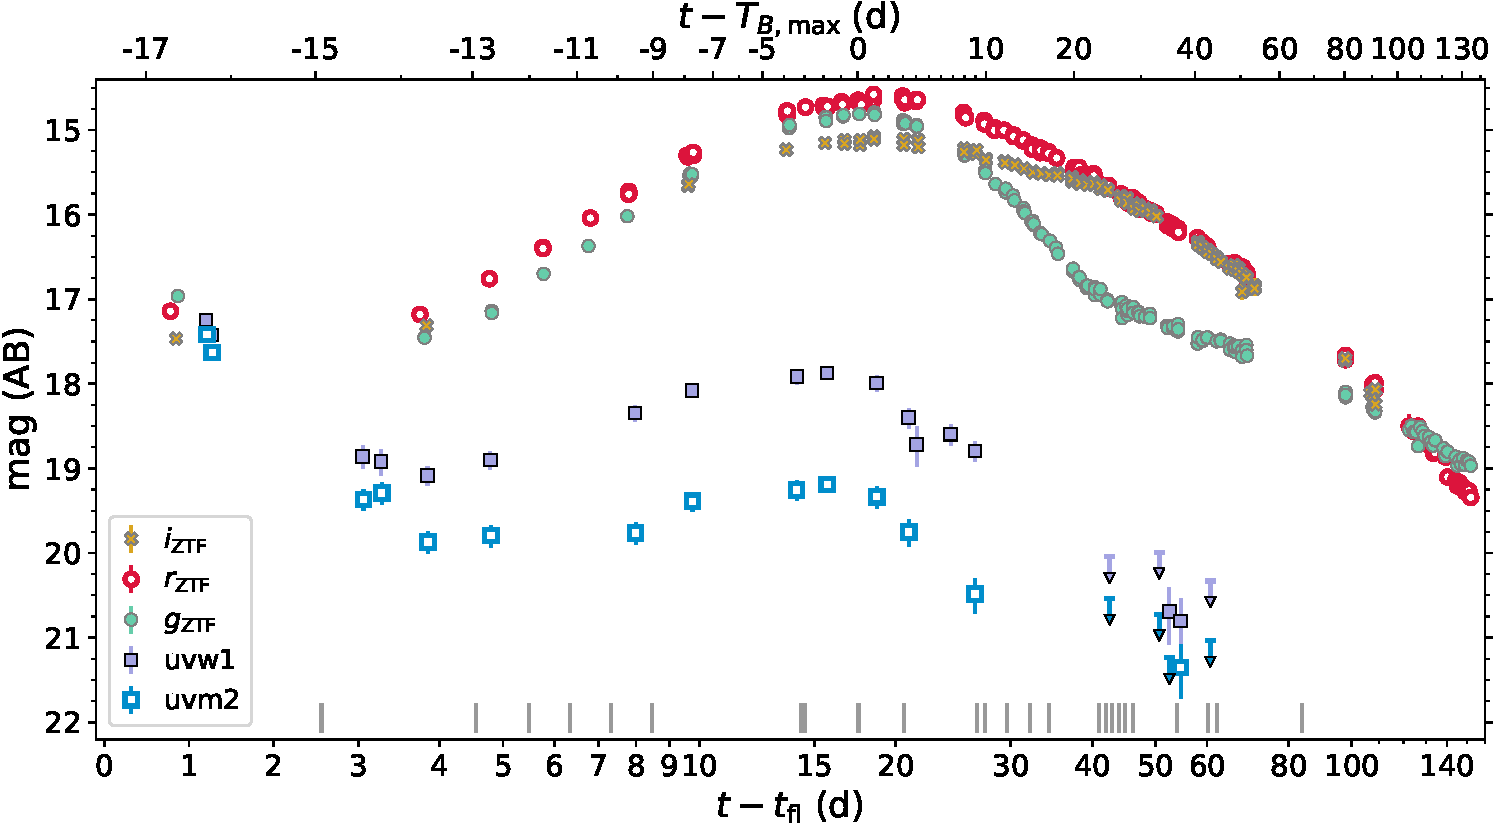
\includegraphics[width=6in]{./figures/P48_lc.pdf}
    %
    \caption{Photometric evolution of \sn, highlighting the initial decline
    observed in the light curve. \gztf, \rztf, and \iztf\ observations are
    shown as filled green circles, open red circles, and filled golden
    crosses, respectively. UVOT $uvw1$ and $uvm2$ are shown as filled and
    open squares, respectively. The lower axis shows time measured in
    rest-frame days relative to the time of first light, \tfl\ (see
    \S\ref{sec:phot}), while the upper axis shows time relative to the time
    of $B$-band maximum, \tbmax. Note that the horizontal axis is shown with
    a linear scale from $0\,\mathrm{d} \le t - t_\mathrm{fl} \le 3$\,d and a
    log scale for $t - t_\mathrm{fl} > 3$\,d. Vertical grey ticks show
    epochs of spectroscopic observations.}
    %
    \label{fig:p48}
\end{figure*}

The field of \sn\ was additionally observed by ZTF with nearly a nightly
cadence as part of the ZTF partnership Uniform Depth Survey (ZUDS;
D.~Goldstein et al., in prep.). Using images obtained as part of the ZUDS
program, we perform forced PSF photometry at the location of \sn\ following
the procedure described in \citet{Yao19}.\footnote{Images obtained as part of
the ZTF public survey have not been released, preventing us from applying our
forced-PSF measurements. We therefore only include forced-PSF measurements in
the analysis described herein, though we note that our measurements are
largely consistent with those provided in the public alerts.} The evolution
of \sn\ in the \gztf, \rztf, and \iztf\ filters is shown in
Figure~\ref{fig:p48}.

\subsection{\textit{Swift} UVOT and XRT Observations}\label{sec:swift}

Ultraviolet (UV) observations of \sn\ were obtained with the
Ultra-Violet/Optical Telescope (UVOT; \citealt{Roming05}) onboard the Neil
Gehrels Swift Observatory (hereafter \textit{Swift}; \citealt{Gehrels04})
following a time-of-opportunity request.\footnote{\textit{Swift} ToO requests
for \sn\ (\textit{Swift} Target ID: 13037) were submitted by
D.~Hiramatsu, J.~Burke, and S.~Schulze.} Pre-SN UVOT reference images are
limited to the $uvw1$, $uvm2$, and $uvw2$ filters. As a result we cannot
provide accurate estimates of the SN flux in the \textit{Swift} $u$, $b$, and
$v$ filters. We estimate the flux in the $uvw1$, $uvm2$, and $uvw2$ filters
using a circular aperture with a $3\arcsec$ radius at the SN position, and
subtract the flux measured using an identical procedure in the pre-SN\,Images.
For clarity, we only show the \textit{Swift} $uvw1$ and $uvm2$ light curves in
Figure~\ref{fig:p48}.\footnote{The $uvw2$ evolution is nearly identical to
$uvm2$. Furthermore, the red leak associated with the $uvw2$ filter (see e.g.,
\citealt{Breeveld11}), in combination with the relatively red spectral energy
distribution of SNe\,Ia, make it very difficult to interpret $uvw2$ light
curves of SNe\,Ia (see \citealt{Brown17} and references therein). Therefore,
unless otherwise noted, we exclude $uvw2$ measurements from the analysis
below.} \textit{Swift}/UVOT observations show that the initial decline seen in
the optical is even more dramatic in the UV.

While absolute flux measurements in the UVOT $u$, $b$, and $v$ filters are
not available, assuming the underlying flux from the host is constant, we
can estimate the time of $B$-band maximum, \tbmax, from the relative
$b$-band light curve. Using a second-order polynomial, we model the $b$-band
light curve near peak (including observations between JD$\,> \,$2,458,855.5
and JD$\,<\,$2,458,871.5). From this fit we estimate \tbmax$ =
$2,458,863.83$ \,\pm \,0.21$\,JD.

In parallel with the \textit{Swift}/UVOT observations, \textit{Swift} observed
\sn\ with its onboard X-ray telescope \citep[XRT;][]{Burrows05} between 0.3
and 10\,keV in the photon counting mode. We analyzed the data with the
online-service of the UK \textit{Swift}
team\footnote{\href{https://www.swift.ac.uk/user_objects/}{\url{https://www.swift.ac.uk/user_objects/}}} that uses the methods described in \citet{Evans07}
and \citet{Evans09} and the software package \texttt{HEASOFT}\footnote{
\href{https://heasarc.gsfc.nasa.gov/docs/software/heasoft/}{\url{https://heasarc.gsfc.nasa.gov/docs/software/heasoft/}}} version 6.26.1 \citep{Heasarc}.

\begin{deluxetable}{rDD}
\tabletypesize{\scriptsize}
\tablewidth{0pt}
\tablecaption{\textit{Swift}/XRT photometry\label{tab:xrt}}
\tablehead{
\colhead{Phase} &
\multicolumn2c{Count Rate} &
\multicolumn2c{Flux} \\
\colhead{(ks)} &
\multicolumn2c{($10^{-3}$\,ct\,s$^{-1}$)} &
\multicolumn2c{$(10^{-14}\,\mathrm{erg\,cm}^{-2}\,\mathrm{s}^{-1})$}
}
\decimals
\startdata
250  &    1.6  $^{+0.6}_{-0.5 }$ &     5.4 $^{+2.1}_{-1.7}$ \\
750  &    1.3  $^{+0.8}_{-0.6 }$ &     4.5 $^{+2.7}_{-2.0}$ \\
1250 &    2.0  $^{+1.1}_{-0.8 }$ &     6.9 $^{+3.9}_{-2.9}$ \\
1750 &    3.3  $^{+1.9}_{-1.4 }$ &    11.4$^{+6.6}_{-4.9}$ \\
2250 & $<$5.4                    & $<$18.8         \\
3750 &$<$17.9                    & $<$62.7         \\
4250 &    2.6  $^{+1.7}_{-1.2 }$ &     8.9$^{+5.8}_{-4.1}$ \\
4750 &    2.2  $^{+1.5}_{-1.1 }$ &     7.8$^{+5.3}_{-3.8}$ \\
5250 & $<$8.4                    & $<$29.3         \\
\enddata
\tablecomments{The count rate and flux are reported in the passband from 0.3 to 10~keV. The flux is corrected for absorption. The reference time is MJD=58846.895949 (29 December 2019 at 21:30:15 UT).}
\end{deluxetable}

To build the light curve, we divided the time-interval of the \textit{Swift}
campaign into blocks of 500\,ks (i.e., 5.8\,d). Table~\ref{tab:xrt} summarizes
our measurements within these intervals, where the photon count rate varies
between 0.001 and 0.003\,ct\,s$^{-1}$, with a signal-to-noise ratio between
$\sim$2.6 and 3.4. In three of these binned epochs we do not detect any
significant X-ray emission, and therefore report $3\sigma$ upper limits. To
convert the count-rate to flux, we build a spectrum from the entire data set
and model the data as an absorbed power-law. In this model, the absorption
components reflect the Galactic absorption towards \sn\ ($N_{\rm
H,\,X}=2.28\times10^{20}\,{\rm cm}^{-2}$)) (unclear where this value comes
from. doesn't match nH column density calculator) and the absorption in the
host galaxy. The photon index $\Gamma$ of the power law ($f \propto
E^{-\Gamma}$) is $2.0^{+0.9}_{-0.5}$ and the host absorption is
$7^{+207}_{-7}\times10^{20}\,{\rm cm}^{-2}$ (90\% confidence). The goodness of
fit is $\chi^2=30.33$ for 31 degrees of freedom
(w-statistics\footnote{\href{http://heasarc.gsfc.nasa.gov/xanadu/xspec/manual/XSappendixStatistics.html}{\url{http://heasarc.gsfc.nasa.gov/xanadu/xspec/manual/XSappendixStatistics.html}}}). The unabsorbed energy conversion factor is
$3.5\times10^{-11}~\mathrm{erg\,cm}^{-2}\,\mathrm{ct}^{-1}$.

Given the constant X-ray emission (to within the uncertainties, see
Table~\ref{tab:xrt}), we conclude that this emission is from a background
source, and not \sn. A lack of X-ray emission is consistent with SNe\,Ia (e.g.,
\citealt{Margutti12}).

\subsection{Optical Spectroscopy}

Spectroscopic observations of \sn\ were initiated because the transient passed
the threshold criteria for both the ZTF Bright Transient Survey
\citep{Fremling19a} and the ZTF Census of the Local Universe experiment
\citep{De20}. Our first spectra was obtained $\sim$2\,d after discovery;
additional spectroscopy was obtained with a variety of telescopes and
instruments over the following $\sim$80\,d. An observing log is listed in
Table~\ref{tab:spectra}. The spectra were reduced using standard procedures in
\texttt{IDL}/\texttt{Python}/\texttt{Matlab}. The optical spectral evolution
of \sn\ is illustrated in Figure~\ref{fig:spec_evo}.

\begin{deluxetable}{lrccc}
\tabletypesize{\scriptsize}
\tablewidth{0pt}
\tablecaption{Spectroscopic Observations of \sn\label{tab:spectra}}
\tablehead{
\colhead{$t_\mathrm{obs}$} &
\colhead{Phase} &
\colhead{Telescope/} &
\colhead{R} &
\colhead{Range} \\
\colhead{(MJD)} &
\colhead{(d)} &
\colhead{Instrument} &
\colhead{$(\Delta\lambda/\lambda)$} &
\colhead{(\AA)}
}
\startdata
58848.27 & $-$14.9 & LT/SPRAT & 350 & 4040--7970 \\
58851.21 & $-$12.0 & LT/SPRAT & 350 & 4040--7970 \\
58852.07 & $-$11.2 & LT/SPRAT & 350 & 4040--7970 \\
58853.07 & $-$10.2 & LT/SPRAT & 350 & 4040--7970 \\
58854.22 &  $-$9.0 & LT/SPRAT & 350 & 4040--7970 \\
58860.13 &  $-$3.2 & LT/SPRAT & 350 & 4040--7970 \\
58860.34 &  $-$3.0 & P60/SEDM & 100 & 3850--9150 \\
58863.38 &  $+$0.0 & P60/SEDM & 100 & 3850--9150 \\
58866.50 &  $+$3.1 & MMT/Binospec & 4000 & 4645--6155 \\
58872.61 &  $+$9.2 & Keck-I/LRIS & 1100 & 3200--10250 \\
58873.30 &  $+$9.9 & P60/SEDM & 100 & 3850--9150 \\
58875.54 & $+$12.1 & P60/SEDM & 100 & 3850--9150 \\
58878.09 & $+$14.6 & NOT/ALFOSC & 360 & 3760--9620 \\
58880.39 & $+$16.9 & P60/SEDM & 100 & 3850--9150 \\
58887.10 & $+$23.5 & LT/SPRAT & 350 & 4040--7970 \\
58888.07 & $+$24.5 & LT/SPRAT & 350 & 4040--7970 \\
58888.97 & $+$25.4 & LT/SPRAT & 350 & 4040--7970 \\
58892.25 & $+$28.6 & P60/SEDM & 100 & 3850--9150 \\
58900.22 & $+$36.5 & P60/SEDM & 100 & 3850--9150 \\
58906.45 & $+$42.7 & P200/DBSP & 700 & 3410--9995 \\
58908.32 & $+$44.6 & P60/SEDM & 100 & 3850--9150 \\
58930.47 & $+$66.5 & Keck-I/LRIS & 1100 & 3200--10250 \\
\enddata
\tablecomments{Phase is measured relative to \tbmax\ in the SN rest frame.
}
\end{deluxetable}

\begin{figure}
    \centering
    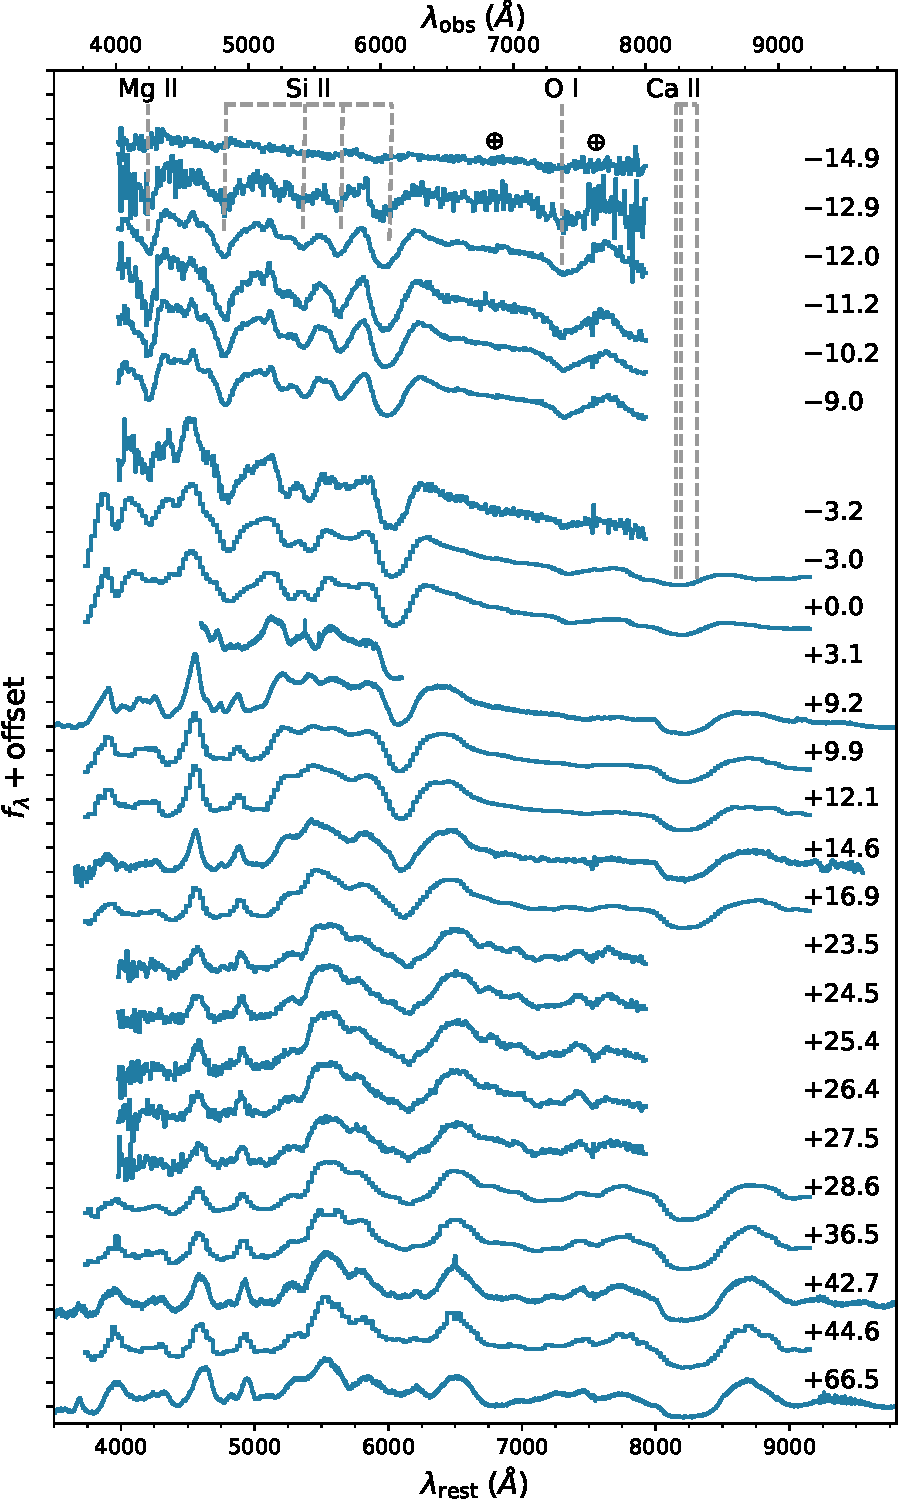
\includegraphics[width=3.35in]{./figures/spec_evo.pdf}
    %
    \caption{Observed spectral sequence of \sn. Spectra have been normalized
    by their median flux between 7200\,\AA\ and 7400\,\AA. The phase of each
    observation relative to \tbmax\ is shown to the right of the individual
    spectra. Prominent spectral features from intermediate mass elements are
    highlighted with vertical dashed lines. Some of the spectra show
    imperfect Telluric subtractions, giving rise to the non-smooth features
    around $\lambda_\mathrm{obs} \approx 7600$\,\AA.}
    %
    \label{fig:spec_evo}
\end{figure}

\section{NGC\,4441: the Host of \sn}\label{sec:host}

NGC\,4441 is the host galaxy of \sn. Sloan Digital Sky Survey (SDSS;
\citealt{York00}) spectroscopic measurements of the nucleus of NGC\,4441
yield a heliocentric-recession velocity of 2663\,\kms\ ($z_\mathrm{helio} =
0.00888$; \citealt{Abolfathi18}) and a \texttt{STARBURST} classification for
NGC\,4441. Morphologically, NGC\,4441 is classified as a peculiar,
weakly-barred, late-type lenticular galaxy (SABO$+$ pec;
\citealt{de-Vaucouleurs91}). SDSS images show a clear dust lane near the
center of the galaxy.

Using the 2M++ model of \citet{Carrick15}, we estimate a peculiar velocity
towards NGC\,4441 of $+328.6$\,\kms, which combined with the recession
velocity in the frame of the cosmic microwave background\footnote{See
\url{https://ned.ipac.caltech.edu/velocity_calculator}} (CMB, $v_\mathrm{CMB}
= 2770.6$\,\kms), yields a total recession velocity $= 3099.2 \pm 150$\,\kms.
The final uncertainty in the total recession velocity is dominated by
systematic uncertainties in the 2M++ model. We also note that the 2M++
estimate is consistent, to within $\sim$5\%, with the Virgo and Great
Attractor infall models of \citet{Mould00}. Adopting $H_0 =
73$\,\kms\,Mpc$^{-1}$, we estimate the distance to NGC\,4441 to be $42.5 \pm
2.1$\,Mpc, corresponding to a distance modulus of $\mu = 33.14 \pm 0.11$\,mag,
where the uncertainty on $\mu$ is dominated by the uncertainty in the peculiar
velocity correction. We hereafter adopt $33.14 \pm 0.11$\,mag as the distance
modulus to NGC\,4441.\footnote{\citet{Tully13} estimate a significantly
smaller distance to NGC\,4441 ($\mu = 31.43 \pm 0.14$\,mag; $D = 19.0$\,Mpc)
based on surface brightness fluctuation measurements from \citet{Tonry01}. If
NGC\,4441 is at this distance, then \sn\ peaks at $M_g \approx -16.8$\,mag,
which is significantly underluminous for a SN\,Ia. Given that \sn\ has a
normal rise time $t_\mathrm{rise} \approx 18$\,d (\S\ref{sec:phot}),
relatively normal spectra at peak (\S\ref{sec:spec}), and lacks the spectral
signatures of intrinsically faint SNe\,Ia (\S\ref{sec:spec_comp}), it is
highly unlikely that it is a factor of $\sim$10 less luminous in the \gztf\
filter than normal SNe\,Ia. We therefore adopt the larger kinematic distance
to NGC\,4441.}
% \todo{Lots of different catalogs provide
% metallicity for SDSS galaxies, should we report on these results at all?
% Port Z = 0.04 and Granada Z ~0.01, and do not agree, firefly ~ 0.6 0r 0.2
% (solar?) depending on weighting, probably not a great idea} \fromkate{that's
% a reasonable spread in values but likely different calibrations. I don't
% know which one is best or the references for comparing this value to. }

We estimate the total reddening towards \sn\ to be small. There is relatively
little line-of-sight extinction due to the Milky Way, $E(B-V) \approx
0.018$\,mag \citep{Schlafly11, Schlegel98}. Furthermore, we do not find
significant evidence for strong interstellar extinction in NGC\,4441.
Figure~\ref{fig:NaD} highlights the \ion{Na}{I} D absorption in the spectrum
of \sn\ due to gas in NGC\,4441 and the Milky Way from our highest-resolution
spectrum, $R \approx 4000$, obtained with Binospec+MMT. The \ion{Na}{I} D
absorption is weak, and we estimate a total equivalent width (EW) $=
390$\,m\AA\ for NGC\,4441 and $220$\,m\AA\ for the Milky Way. There is a
systematic uncertainty of $\sim$10\% on each of these estimates due to
uncertainties in the continuum-fitting procedure. Assuming similar properties
for the dust in NGC\,4441 and the Milky Way, we scale the color excess
measurement for the Milky Way by the ratio of \ion{Na}{I} D EWs to estimate
$E(B-V) \approx 0.032$\,mag for \sn\ due to interstellar absorption in
NGC\,4441. This yields a total color excess towards \sn\ of $E(B-V) \approx
0.05$\,mag, which we adopt for the subsequent analysis in this study. We note
that this estimate is consistent, to within the uncertainties, with the
EW(\ion{Na}{I} D)--$E(B-V)$ relations presented in \citet{Poznanski12}.
Further supporting the claim of low interstellar extinction in NGC\,4441 is
the lack of a detection of the \ion{K}{I} $\lambda\lambda$7665, 7699
interstellar lines or the diffuse interstellar band at 5780\,\AA, which also
serve as proxies for extinction (e.g., \citealt{Phillips13}).

\begin{figure} \centering 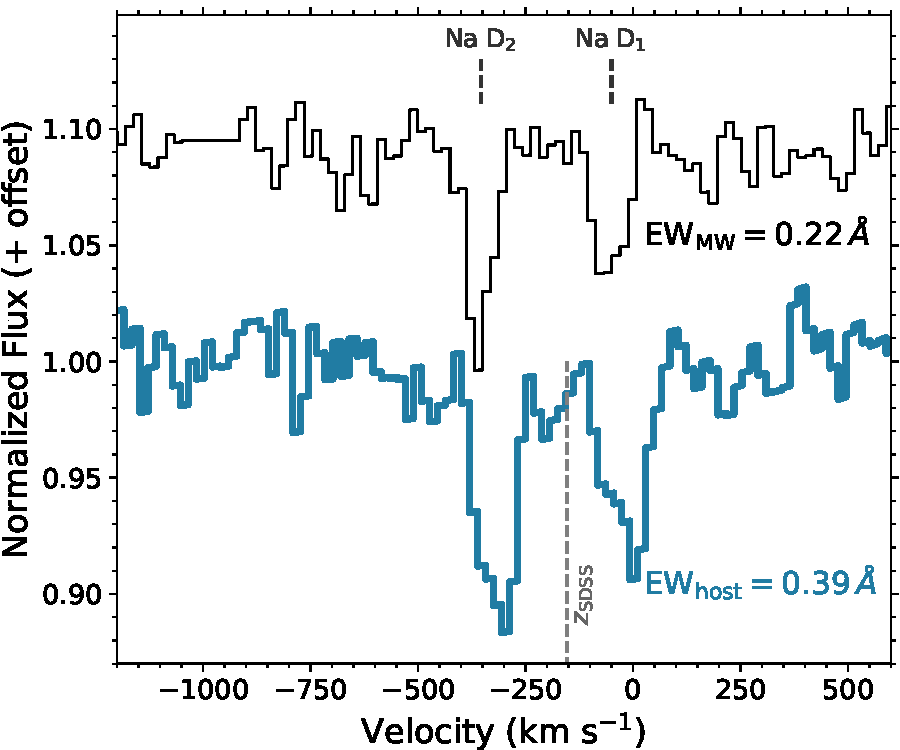
\includegraphics[width=3.35in]{./figures/NaD.pdf}
    %
    \caption{Zoom in on our moderate resolution ($R \approx 4000$)
    MMT+Binospec spectrum of \sn\ highlighting absorption due to \ion{Na}{I} D
    in the host galaxy, NGC\,4441 (blue solid line), and the Milky Way (thin
    black line). The velocity scale is centered on the D$_1$ line in
    NGC\,4441, with the SDSS redshift shown via the vertical dashed line. The
    velocity scale is centered on 5895.92\,\AA\ for the Milky Way absorption
    lines. The \ion{Na}{I} D lines, which serve as a proxy for interstellar
    dust-obscuration along the line of sight (e.g.,
    \citealt{Poznanski12,Phillips13}) are weak, indicating a relatively small
    amount of reddening.}
    %
    \label{fig:NaD}
\end{figure}



\section{Photometric Analysis}\label{sec:phot}

\subsection{The Time of First Light, \tfl}\label{sec:t_fl}

We estimate the time of first light, \tfl, for \sn\ following the procedure
described in \citet{Miller20}. Briefly, \citet{Miller20} model the early
emission from a SN\,Ia as a power-law in time, $f \propto (t -
t_\mathrm{fl})^\alpha$, where $f$ is the flux, $t$ is time, and $\alpha$ is
the power-law index. \tfl\ is assumed to be the same everywhere in the
optical, allowing us to simultaneously fit observations in each of the ZTF
filters.

An important caveat for \sn\ is that the observed early decline in the light
curve clearly does not follow the simple power-law model, and thus these
observations must be masked when performing the fit. We conservatively exclude
observations from the first two nights of ZTF detection from the fit (this
choice is conservative as it is unclear when the mechanism that powers the
initial bump in \sn\ no longer significantly contributes to the flux in the
\gztf\ and \rztf\ filters). From the fit we find \tfl$ = -17.5
\pm^{1.0}_{1.3}$\,d relative to \tbmax. We know that the time of explosion
must be $< -17.4$\,d based on the discovery detection in \citealt{Itagaki19},
and, by definition $t_\mathrm{fl} \ge t_\mathrm{exp}$, meaning a portion of
the posterior distribution for our model cannot be correct. We find $\alpha_g
= 2.15 \pm^{0.49}_{0.36}$ and $\alpha_r = 1.91 \pm^{0.42}_{0.31}$, which are
typical of the normal SNe Ia studied in \citet{Miller20}. If we only exclude
the first observation from the model fit we find significantly different
results with a rise time that increases by $\sim$5\,d and power-law indices
that increase by $\gtrsim 1$. We note that such a long rise is unlikely,
however, as our spectroscopic models (see \S\ref{sec:tardis}) estimate the
time of explosion, $t_\mathrm{exp}$, to be $\sim$17.9\,d prior to \tbmax,
fully consistent with our estimate of \tfl.

% \fromkate{The rise time is long for its magnitude and stretch. From
% \citet{Gonzalez-Gaitan12}, the risetime would suggest a high stretch event,
% their fig. 12. Likely just the impact of the early component but worth
% stressing. }

\subsection{Luminosity of the Initial UV/optical Flash}\label{sec:luminosity}

To estimate the luminosity and temperature of the initial UV/optical flash
from \sn, we model the broadband spectral energy distribution (SED) as a
blackbody. The assumed distance and reddening towards \sn\ are taken from
\S\ref{sec:host}. The ZTF optical and \textit{Swift} UV observations were not
simultaneous, so we therefore interpolate the optical light curves to estimate
the flux during the same epochs as \textit{Swift} observations. While SNe\,Ia
do not emit as pure blackbodies, our initial spectrum of \sn\ shows a blue and
nearly featureless continuum largely consistent with blackbody emission. The
blackbody assumption is therefore reasonable for the early flash from \sn,
which is distinctly different from normal SNe.

Following interpolation to an epoch 1.24~rest-frame~d after \tfl\
($\mathrm{JD} = $2,458,847.43), we estimate a blackbody luminosity $L = (1.7
\pm ^{0.2}_{0.1}) \times 10^{42}$\,erg\,s$^{-1}$ and temperature
$T_\mathrm{eff} = 14.8 \pm^{0.9}_{1.2}$\,kK. This estimate represents a lower
limit to the peak luminosity of the initial flash, as the UV flux was already
decreasing at this time (\textit{Swift} obtained two sets of UV observations
separated by $\sim$90\,min during the first epoch of observations, and the
$uvm2$ and $uvm1$ flux is clearly decreasing during this time; see
Figure~\ref{fig:p48}). 

At an epoch 3.15~rest-frame~d after \tfl, we estimate the luminosity and
temperature to have fallen to $L = (7.0 \pm ^{0.9}_{0.6}) \times
10^{41}$\,erg\,s$^{-1}$ and $T_\mathrm{eff} = 8.7 \pm^{0.5}_{0.4}$\,kK,
respectively. For this epoch we have excluded the $uvw2$ flux from the
blackbody model due to the significantly lower temperature, and known red leak
for that filter (see \S\ref{sec:swift}). This measurement of $T_\mathrm{eff}$
is consistent with our model spectrum from 2.6~rest-frame~d after \tfl (see
\S\ref{sec:tardis}). At a similar epoch, $\sim$4\,d after explosion,
\citet{Cao15} estimate a UV flash luminosity of $\sim$3$ \times
10^{41}$erg\,s$^{-1}$ in iPTF\,14atg, a factor of $\sim$2 less than for \sn.
% 19yvq max luminosity ~ 1.95e9 Lsun (5.4 -- 7.5e42)
% 14atg max luminosity ~ 3.8e42 -- from Kromer

Finally, if we conservatively assume that the early flash peaked 1\,d after
\tfl\ (i.e., at the epoch of the first \textit{Swift} observation), and
abruptly ended 3\,d after \tfl\ (i.e., at the epoch of the second
\textit{Swift} observation), then the initial flash emitted a total integrated
energy of $\sim$4$\times 10^{42}$\,erg.
% flash peak ~ 1.82e42; total = 1.82e42/2 + 2*7e41 + 2*1.12e+42/2
These assumed times are highly uncertain, however, it is likely that the SN
exploded before \tfl\ (see e.g., \S\ref{sec:companion_interaction}), and the
UV flux continues to decline $>$3\,d after \tfl\ (Figure~\ref{fig:p48})
suggesting the flash lasted longer than 3\,d.

\subsection{Maximum Light and Decline}\label{sec:max_decline}

While the rise time and power-law indices of \sn\ are similar to other normal
SNe Ia, the full photometric evolution does not resemble a normal SN\,Ia. The
photometric evolution of \sn\ is highlighted in Figure~\ref{fig:lc_comp},
where \sn\ is compared to 121 normal SNe\,Ia from \citet{Yao19}.\footnote{For
the purposes of this comparison we consider SN\,1991T-like, SN\,1999a-like,
and SN\,1986G-like events to all be normal SNe\,Ia.} \sn\ is somewhat
underluminous ($M_{g,\mathrm{max}} \approx -18.5$\,mag), declines rapidly
($\Delta m_{15}(g) = 1.30\pm^{0.01}_{0.02}$\,mag, uncertainties represent the
68\% credible region), and does not exhibit a ``shoulder'' in the \rztf\ or a
strong secondary maximum in the \iztf\ light curves post-maximum. The slightly
underluminous and moderately fast decline of \sn\ are very similar to the
SN\,1986G-like SNe\,Ia, which represent a transitional group between normal
SNe\,Ia and the underluminous SN\,1991bg-like class (e.g.,
\citealt{Taubenberger17} and references therein). While the photometric
evolution of \sn\ is similar to 86G-like SNe, we show that \sn\ is
spectroscopically distinct from these transitional SNe
(\S\ref{sec:spec_comp}).

\begin{figure}
    \centering
    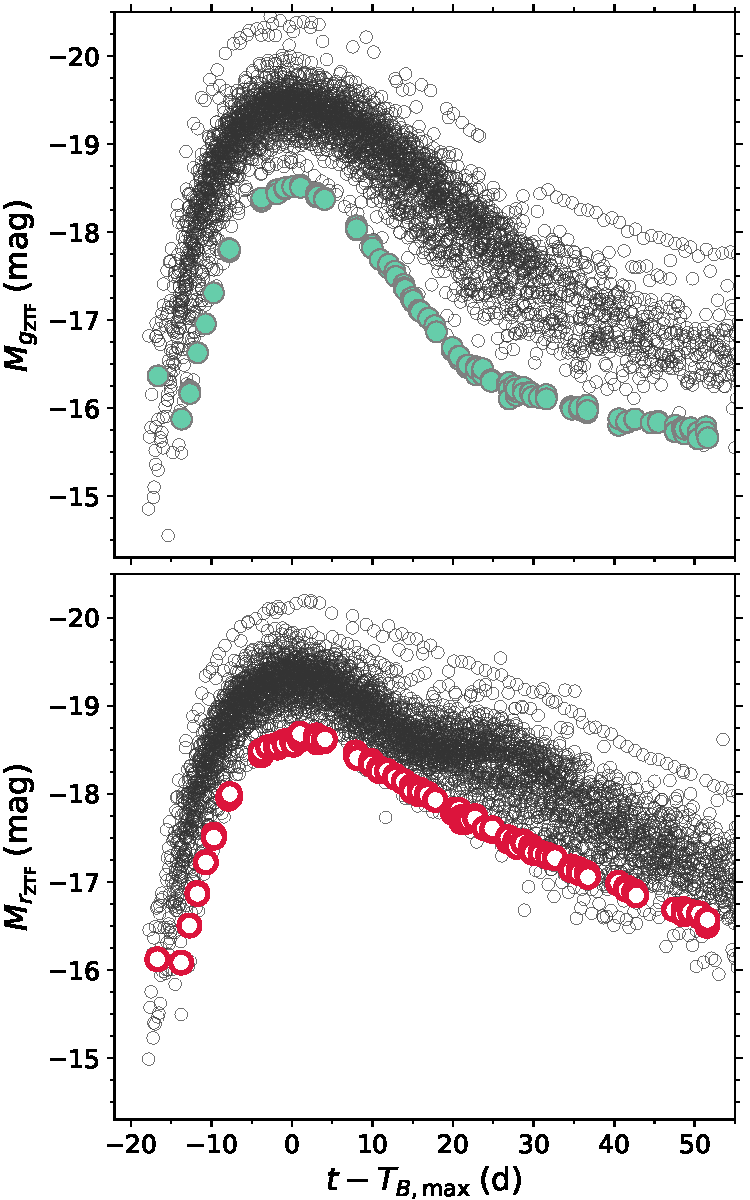
\includegraphics[width=3.35in]{./figures/abs_mag_host_ebv_kcorr.pdf}
    %
    \caption{Photometric evolution of \sn\ compared to 121 normal SNe\,Ia
    observed by ZTF \citep{Yao19} in the \gztf\ (\textit{top}) and \rztf\
    (\textit{bottom}) filters. The normal SNe are shown as open grey circles,
    while the symbols for \sn\ are the same as Figure~\ref{fig:p48}. Relative
    to normal SNe\,Ia, \sn\ is fainter, declines faster in \gztf, and lacks
    the ``shoulder'' typically seen in the \rztf\ filter. Normal SNe light
    curves have been corrected for host-galaxy reddening and $K$-corrections
    have been applied, with both determined via \texttt{SNooPY} (see
    \citealt{Bulla20} for details of our implementation). $K$-corrections have
    not been applied to the light curve of \sn.}
    %
    \label{fig:lc_comp}
\end{figure}

% For context, of the 127 SNe\,Ia observed by ZTF and studied in \citet{Yao19}, only 1, ZTF18abclfee (SN\,2018crl), a SN\,2002cx-like event, had a faster decline than \sn. and, according to the new photometric classification scheme presented in \citet{Ashall20}, \sn\ is consistent with  91bg-like SNe.

We also find that standard SN\,Ia fitting techniques do not provide good
matches to the evolution of \sn. For example, a \texttt{SNooPY}
\citep{Burns11} fit to the optical light curve requires significant
host-galaxy extinction ($E(B-V)_\mathrm{host}\approx0.4$\,mag, cf.\
\S\ref{sec:host}) to match the observed red colors, while predicting a
secondary maximum in the \iztf-band and a fast evolution after peak that is
not seen in \sn. A \texttt{SALT2} \citep{Guy07} fit leads to similar
inconsistencies to those in \texttt{SNooPy}. These inconsistencies support our
conclusion above that the photometric evolution of \sn\ does not match normal
SNe\,Ia.

\subsection{Color Evolution}

\sn\ is further distinguished from normal SNe Ia by its unusual color
evolution (Figure~\ref{fig:colors}). The top panel of Figure~\ref{fig:colors}
shows the \gztf$ - $\rztf\ evolution of 62 spectroscopically normal SNe Ia
with ZTF observations within 5\,d of \tfl\ (see \citealt{Bulla20}), with the
color evolution of \sn\ over-plotted. The initially blue colors in \sn\
rapidly evolve to the red over the first few days of observation before
gradually becoming bluer in the time leading up to \tbmax\ (this behavior is
deemed an early ``red bump'' in \citealt{Bulla20}). Similar red bumps are only
seen in 6 of the 62 normal SNe\,Ia ($\sim$10\%) in the ZTF sample
\citep{Bulla20}, and they are typically less pronounced than what is observed
in \sn.

Furthermore, while normal SNe Ia exhibit a large scatter in
\gztf$ - $\rztf\ shortly after \tfl\ they evolve to form a tight locus between
$\sim$10--30\,d after \tfl. \sn\ is redder at peak than each of the normal SNe
Ia in the \citet{Bulla20} sample. Post maximum, only 1 normal SN\,Ia,
ZTF\,18abeegsl (SN\,2018eag), exhibits a similarly radid decline in \gztf$ -
$\rztf\ color. The \gztf$ - $\rztf\ color evolution of \sn\ is again
intermediate between normal SNe\,Ia and underluminous 91bg-like SNe.
Figure~\ref{fig:colors} shows that normal SNe\,Ia are reddest at $\sim$+30\,d,
while 91bg-like SNe are reddest between $\sim$+10--15\,d \citet{Burns14}. \sn\
reaches a \gztf$-$\rztf\ maximum at an intermediate time of $\sim$+20\,d.

\begin{figure}
    \centering
    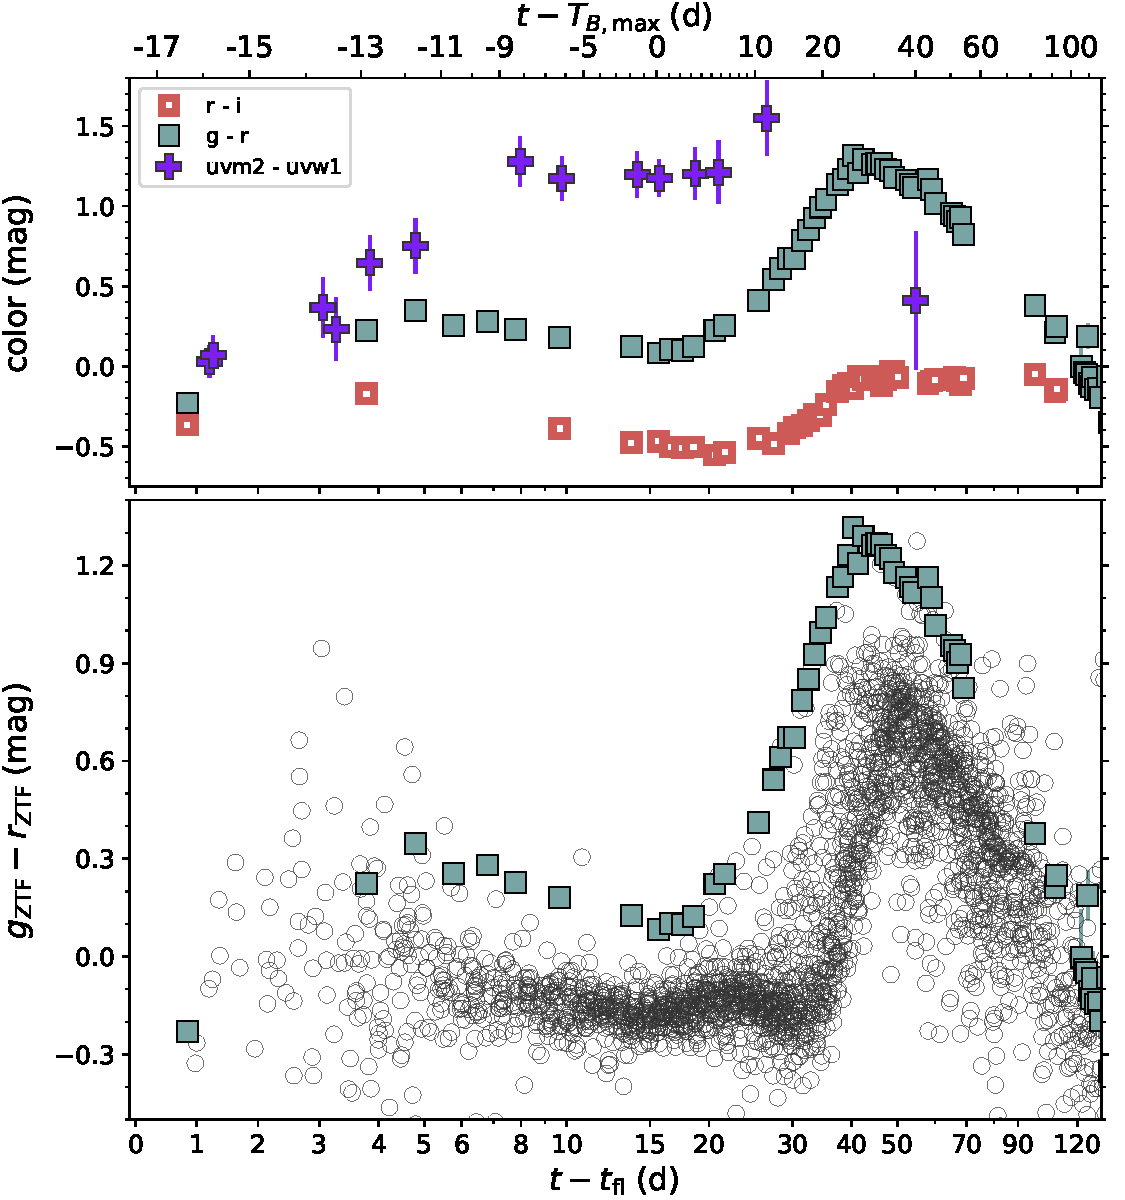
\includegraphics[width=3.35in]{./figures/P48_colors.pdf}
    %
    \caption{Photometric color evolution of \sn\ relative to \tfl\ (the
    timescale relative to \tbmax\ shown along the top axis only applies to
    \sn). \textit{Top}: \gztf$ - $\rztf\ evolution of \sn\ (solid green
    squares), corrected for the total interstellar extinction (see
    \S\ref{sec:host}), and compared with the evolution of 62 normal SNe Ia
    (open circles) observed within 5\,d of \tfl\ by ZTF (from
    \citealt{Bulla20}). \sn\ is the reddest SN in the group, and it exhibits
    the fastest evolution to red colors post-\tbmax. \textit{Bottom}: the
    $uvm2 - uvw1$ (purple crosses), \gztf$ - $\rztf\ (solid, green squares),
    and \rztf$ - $\iztf\ (open, red squares) color evolution of \sn.}
    %
    \label{fig:colors}
\end{figure}

The offset in the \gztf$ - $\rztf\ color evolution of \sn\ relative to normal
SNe\,Ia would be reduced if the reddening towards \sn\ has been significantly
underestimated. A color excess of $E(B-V) \approx 0.25$\,mag, rather than the
0.05\,mag adopted in \S\ref{sec:host}, would roughly align the pre-\tbmax\
\gztf$ - $\rztf\ color of \sn\ with the tight locus seen in
Figure~\ref{fig:colors}. Such a correction would also bring the peak optical
brightness of \sn\ in line with normal SNe\,Ia [for $E(B-V) \approx
0.25$\,mag, $M_g \approx -19.25$\,mag and $M_r \approx -19.1$\,mag for \sn].

While the spectral appearance of \sn\ is similar to some normal SNe\,Ia (see
\S\ref{sec:spec_comp}), the observed rapid decline in the \gztf\ filter
provides strong evidence that \sn\ is not a normal luminosity SN\,Ia.
\citet{Phillips93} showed that in the optical SNe\,Ia follow a
brightness--width relation, whereby brighter explosions decline less rapidly.
Thus, with a typical peak in the optical, as would be implied with $E(B-V)
\approx 0.25$\,mag, the fast decline in \sn\ [$\Delta m_{15}(g) = 1.3$\,mag]
would be largely unprecedented.\footnote{Only 2 spectroscopically normal
SNe\,Ia in the \citet{Yao19} sample decline faster than \sn\ as measured by
$\Delta m_{15}(g)$. While the lack of \textit{Swift} $b$-band templates
prevents us from measuring $\Delta m_{15}(B)$, the relationship between that
and $\Delta m_{15}(g)$ for normal ZTF SNe\,Ia suggests $\Delta m_{15}(B)
\gtrsim 1.6$\,mag for \sn.} This conclusion is further corroborated by the
rapid evolution of the \gztf$-$\rztf\ color to the red after \tbmax\ and the
lack of a secondary maximum in the \iztf-band, each of which is typical of
lower luminosity SNe\,Ia \citep[see][and references therein]{Taubenberger17}.
We therefore conclude that the color excess towards \sn\ is not
underestimated, and that the SN is instead intrinsically red in the optical.

% Such a large reddening would dramatically change the appearance of \sn\ in
% the UV. If we assume $E(B-V) \approx 0.25$\,mag, then the luminosity of the
% initial flash would be $\sim$8.7$\times 10^{42}$\,erg\,s$^{-1}$, more than a
% factor of 5 higher than what we estimated in \S\ref{sec:luminosity}.

% The bottom panel of Figure~\ref{fig:colors} shows the $uvm2 - uvw1$
% color evolution of \sn. At \tbmax, $uvm2 - uvw1 \approx 1.2$\,mag, making
% \sn\ one of the most UV blue SNe\,Ia at maximum light (e.g.,
% \citealt{Milne10,Brown17}). A color excess of $E(B-V) \approx 0.25$\,mag is
% equivalent to $E(uvm2 - uvw1) \approx 0.5$\,mag using the Fitzpatrick+
% (1999) extinction law, $R_V = 3.1$, and the effective wavelengths of the
% \textit{Swift} filters from \citet{Brown17} \frommb{I get 0.65 mag, maybe
% double-check?}. \fromkate{I did this calc, I've checked and using method and
% values listed, I get 0.5 mag for the uvm2-uvw1 colour} This results in a
% $uvm2 - uvw1 \approx 0.XXX$\,mag at \tbmax, making \sn\ the most UV blue
% SN\,Ia observed by \textit{Swift} \fromkate{this needs to be updated because
% none of the objects in Brown sample are corrected for extinction}.

Even if one ignores the striking initial bump in the light curve of \sn, we
can still conclude that \sn\ is not a normal SN\,Ia based on its other
photometric properties (e.g., relatively faint peak optical brightness,
moderately fast decline, lack of a near-infrared secondary maximum, and red
appearance at peak).

\section{Spectral Evolution of \sn}\label{sec:spec}

Optical spectra of \sn\ were obtained at phases from $-$14.9\,d (2.6\,d after
\tfl) to 66.5\,d after \tbmax. Details of the spectra are presented in
Table~\ref{tab:spectra} and the spectral evolution is shown in
Figure~\ref{fig:spec_evo}. Many of the spectra were obtained with the Spectral
Energy Density Machine \citep[SEDM;][]{Blagorodnova18,Rigault19}, which was
designed specifically for SN classification \citep[e.g.,][]{Fremling19a}, yet
for \sn\ the quality is high enough to provide detailed absorption line
measurements (see \S\ref{sec:SiII}). The absorption features in \sn\ are
typical of SNe\,Ia, including intermediate mass elements (IMEs), primarily Si,
Ca, and O, as well as iron-group elements (IGEs).

\subsection{TARDIS Models}\label{sec:tardis}

To determine the structure of the ejecta and relative contributions of
different ions at early and maximum light phases, we have modeled the spectra
at $-$14.9\,d, $-12.0$\,d, and $+$0.0\,d using the 1D Monte Carlo radiative
transfer code \texttt{TARDIS} \citep{Kerzendorf14}. We note that
\texttt{TARDIS} assumes a single, sharp photosphere between the optically
thick and thin regions. Therefore, if there is a contribution to the spectrum
from an underlying quasi-blackbody (at early times this could be due to
interaction, for example; see \S\ref{sec:companion_interaction}), this will
impact the ability of \texttt{TARDIS} to fully reproduce the observations.
Nevertheless, our models should provide a reasonable approximation of the
plasma state within the ejecta. Parameters of our \texttt{TARDIS} models are
given in Table~\ref{tab:tardis}.

\begin{deluxetable*}{lcrrccc}
\tabletypesize{\scriptsize}
\tablewidth{0pt}
\tablecaption{\texttt{TARDIS} input parameters\label{tab:tardis}}
\tablehead{
\colhead{Date} &
\colhead{MJD} &
\colhead{Phase\tablenotemark{a}} &
\colhead{$t - t_\mathrm{exp}$\tablenotemark{b}} &
\colhead{$L$\tablenotemark{c}} &
\colhead{$v_\mathrm{boundary}$\tablenotemark{d} }&
\colhead{$T_\mathrm{boundary}$\tablenotemark{e} } \\
\colhead{(UT) }&
\colhead{} &
\colhead{(d)} &
\colhead{(d)} &
\colhead{($\log L_{\odot}$)} &
\colhead{(\kms) } &
\colhead{(K)}
}
\startdata
2019 Dec 31.277 & 58848.277 & $-14.9$ & 3.0 & 8.55 & 25,000 & 8173 \\
2020 Jan 03.217 & 58851.217 & $-12.0$ & 6.0 & 8.60 & 16,500 & 7925 \\
2020 Jan 15.392 & 58863.392 & $+0.0$ & 18.0 & 9.29 & 10,500 & 9696 \\
\enddata
\tablenotetext{a}{Rest-frame time relative to the time of $B$-band maximum,
\tbmax.}
\tablenotetext{b}{Rest-frame time relative to the \texttt{TARDIS} time of
explosion, $t_\mathrm{exp}$.}
\tablenotetext{c}{Emergent Luminosity.}
\tablenotetext{d}{Ejecta velocity at the inner boundary of the photosphere.}
\tablenotetext{e}{Temperature at the inner boundary of the photosphere. The
inner boundary temperature is not explicitly an input parameter for
\texttt{TARDIS}, it is derived from the luminosity, time since explosion,
inner boundary velocity, and iteratively updated throughout the simulation.}

\end{deluxetable*}

%%%Description of overall modelling results, velocities, features present, temperature. Then detailed discussion of Mg II vs Si III can be removed.
The first spectrum of \sn\ at $-$14.9\,d (2.6\,d after \tfl, 3.0\,d after
explosion) shows shallow features consistent with IMEs moving at extremely
high velocities ($>$\,20,000\,\kms, Figure~\ref{fig:spec_evo}). The
best-fitting \texttt{TARDIS} model is shown in Figure~\ref{fig:tardis}, along
with the contribution of individual elements to the spectral features. For
this model, we have assumed a uniform composition of O, Mg, Si, and S. Our
model demonstrates that the shallow absorption features observed at this phase
can be reproduced solely by IMEs (predominantly \ion{Si}{II}), and that the
presence of IGE is not required to match the data. Our model also confirms the
high velocities of the ejecta -- we find the spectral features and temperature
are best reproduced with a photospheric velocity of
$\sim$25,000\,\kms.

\begin{figure*}
    \centering
    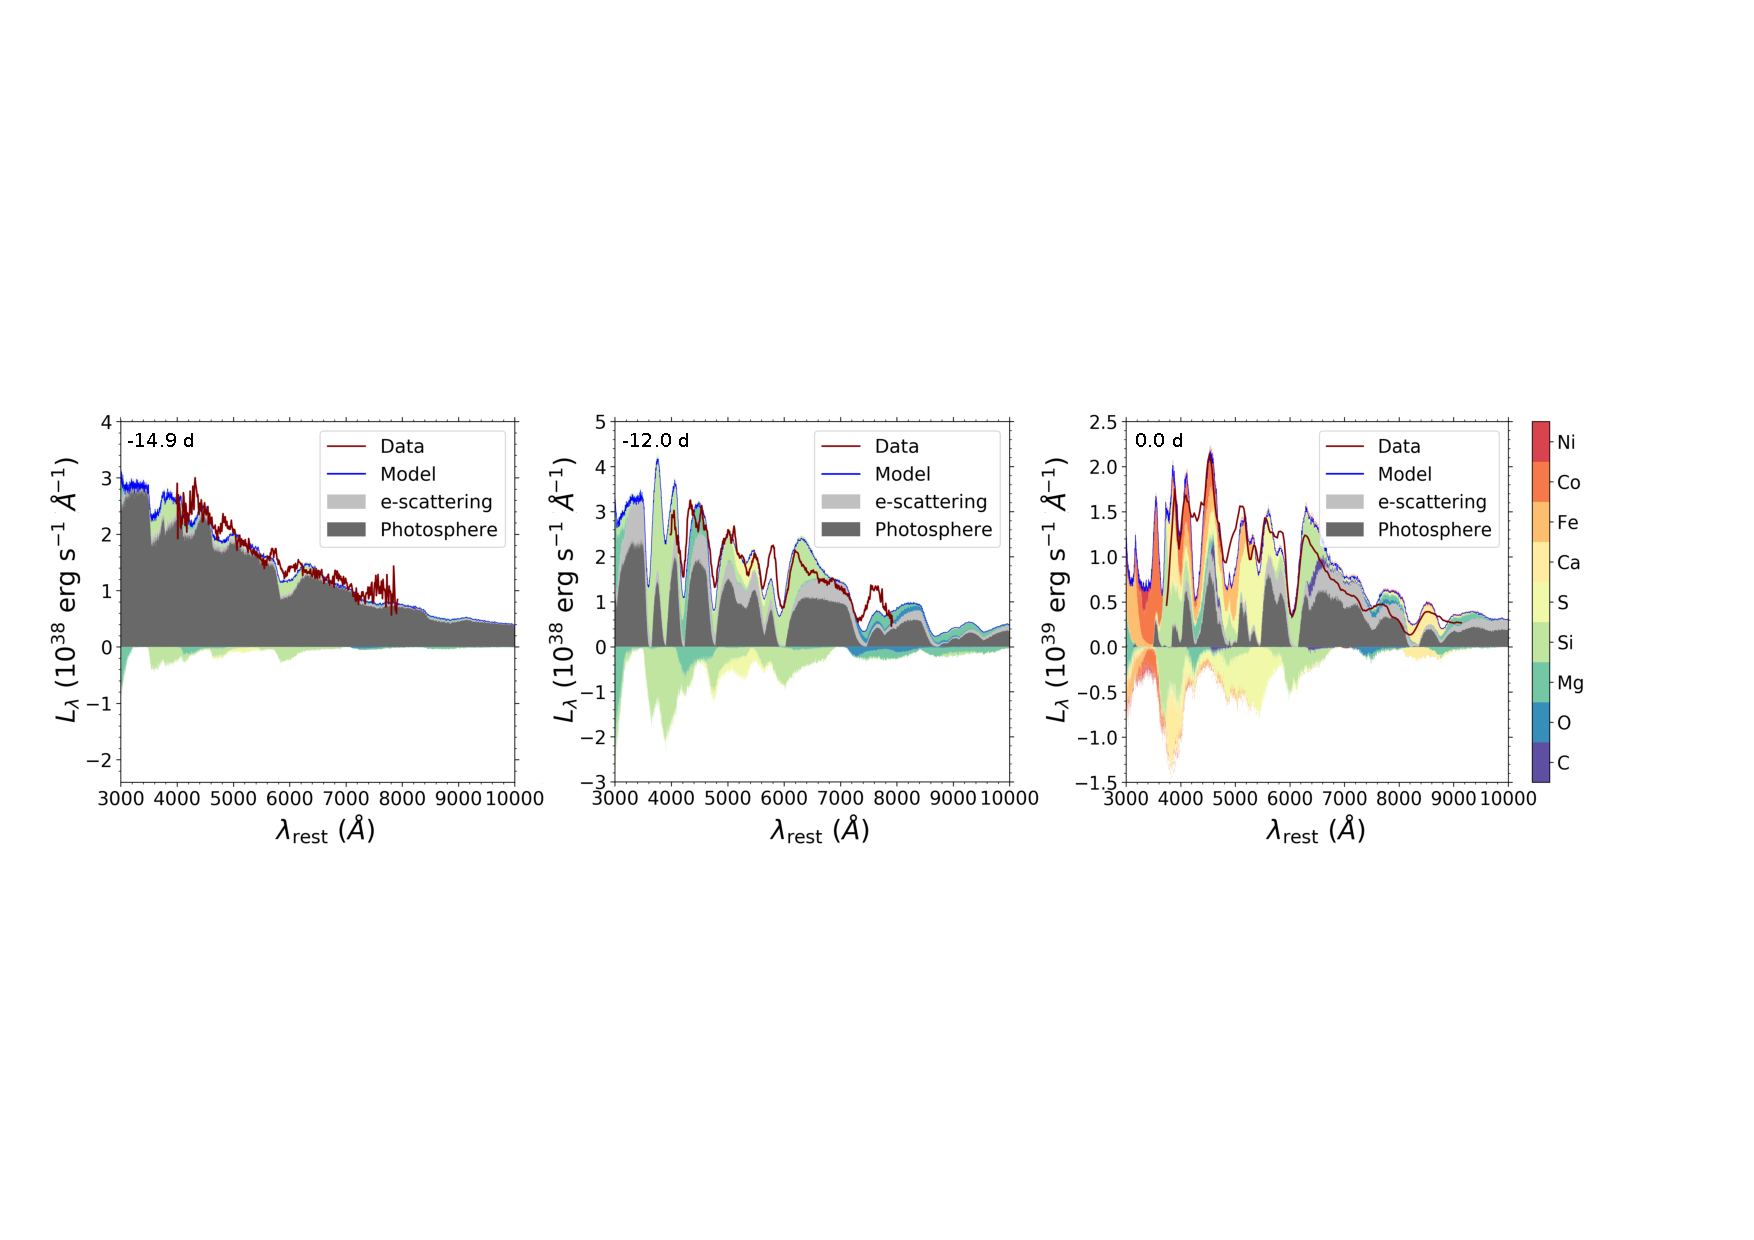
\includegraphics[width=\textwidth]{./figures/tardis.pdf}
    %
    \caption{Comparison of \texttt{TARDIS} models to \sn\ at $-$14.9\,d
    (left), $-12.0$\,d (middle), and $+$0.0\,d (right), relative to \tbmax.
    For each model, we color code a histogram showing the contribution of
    each element to the spectroscopic features, based on the last element with
    which a Monte Carlo packet experienced an interaction. Packets may be
    absorbed and re-emitted at different wavelengths, with the exception of
    those packets that only experience electron scattering. During electron
    scattering, only the direction of propagation is changed. These packets
    are shown in grey. Packets that did not interact during the simulation are
    shown in black. Contributions above/below zero demonstrate the sum of
    packet luminosities after/before their last interaction.}
    %
    \label{fig:tardis}
\end{figure*}

Similarly, for the $-12.0$\,d spectrum we find that a model that does not
contain IGE above $\sim$16,500\,\kms\ reproduces the majority of the
spectroscopic features. Again, our model contains a uniform composition of O,
Mg, Si, and S, and is shown in Figure~\ref{fig:tardis}. At this phase the model
suggests the photospheric temperature has not significantly changed, however
the features have become much more prominent. Compared to modeling of the
spectroscopically similar SN\,2002bo (see \S\ref{sec:spec_comp}) at the same
epoch \citep{Stehle05}, we find \sn\ has a lower photospheric temperature
($\sim$8,000\,K, compared to $\sim$9,500\,K for SN\,2002bo).

While the early spectra of \sn\ are dominated by IMEs, there is no evidence in
the observed spectra for \ion{C}{II} absorption. However, in our
\texttt{TARDIS} models even if we increase the C abundance in the outer ejecta
to large amounts (50\%), the model spectra still lack any significant
\ion{C}{II} features at the time of our observations. Our ability to detect
\ion{C}{II} in the spectra of \sn\ is likely affected by the extremely high
ejecta velocities, which leads to blending with \ion{Si}{II}. Therefore,
despite the lack of a \ion{C}{II} detection in the observed spectra, we are
unable to place meaningful constraints on the C abundance in the very
outermost ejecta.

Given that our $+0$\,d maximum light spectrum occurs 12\,d after our previous
model spectrum, we assume a composition for the inner ejecta
($\textless$16,500\,\kms) similar to that found for SN\,2002bo
\citep{Stehle05}. A more detailed ejecta structure could be achieved through
modeling additional pre-maximum spectra, but is beyond the scope of the work
presented here. As shown in Figure~\ref{fig:tardis}, our model is able to
broadly reproduce many of the features observed. Notable exceptions include
the features around $\sim$4200 and 4900\,\AA, which we attribute to Fe. Better
spectroscopic agreement could potentially be achieved if \sn\ had a lower
abundance of IGE within the inner ejecta relative to SN\,2002bo.

Overall, our \texttt{TARDIS} modeling demonstrates that \sn\ is consistent
with a low (or zero) fraction of IGE in the outer ejecta. Additionally, the
earliest phases show little change in temperature (see
Table~\ref{tab:tardis}), as expected from the color evolution.

\subsection{\ion{Si}{II} Evolution}\label{sec:SiII}

We have measured the velocity of the \ion{Si}{II} $\lambda$6355 absorption
feature following the procedure in \citet[][see their \S2.5]{Maguire14}. We
have also estimated the pseudo-equivalent widths (pEWs) of the \ion{Si}{II}
$\lambda\lambda$5972, 6355 features, allowing us to measure their ratio, also
known as $\mathcal{R}($\ion{Si}{II}$)$; see \citet{Hachinger08} for the
updated definition relative to \citet{Nugent95}.

\begin{figure}
    \centering
    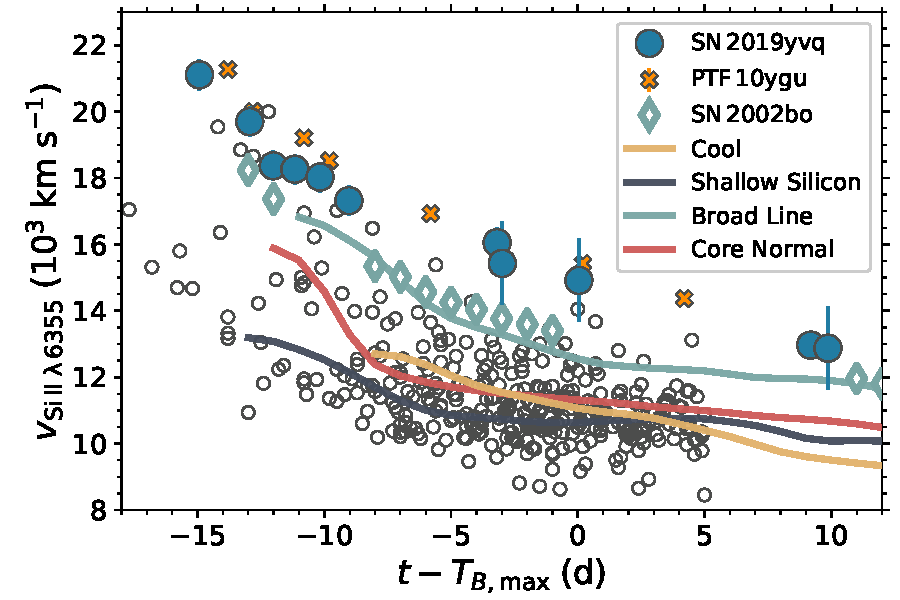
\includegraphics[width=3.35in]{./figures/vel_evolution.pdf}
    %
    \caption{Velocity evolution of \ion{Si}{II} $\lambda$6355 absorption in
    \sn\ (large, filled circles). For comparison we also show the measurements
    for 264 SNe Ia observed by the Palomar Transient Factory \citep[PTF; data
    from][]{Maguire14} as open circles, with SN\,2010jn (PTF\,10ygu), the SN
    with the fastest moving ejecta in the PTF sample, highlighted via orange
    crosses. We additionally show the velocity evolution of SN\,2002bo
    \citep[data from][]{Benetti04}, a SN that is very similar to \sn, as open
    diamonds. The median velocity evolution of each of the spectroscopic
    classes defined by \citet[][Shallow Silicon, Core Normal, Broad Line, and
    Cool]{Branch06} are shown via solid lines. It is clear that \sn\ has
    exceptionally high-velocity ejecta relative to typical SNe Ia.}
    %
    \label{fig:vel_evo}
\end{figure}

%%%Velocity and equivalent width measurements?
The velocity evolution of \ion{Si}{II} $\lambda$6355 is shown in
Figure~\ref{fig:vel_evo}, compared to measurements for the Palomar Transient
Factory (PTF) SN\,Ia sample from \citet{Maguire14} and the median velocity
evolution of SNe\,Ia belonging to the four different classes (Shallow Silicon,
Core Normal, Broad Line, and Cool) identified in
\citet{Branch06};\footnote{The velocity measurements are from
\citet{Blondin12}, while the method to determine the median velocity is
described in \citet{Miller18}.} hereafter, the \citeauthor{Branch06}~class.
The \ion{Si}{II} $\lambda$6355 velocity in \sn\ is $\sim$15,000\,\kms\ around
\tbmax.

At \tbmax, the pEW measurements for the \ion{Si}{II} $\lambda$6355 and
$\lambda$5972 features are $183\pm1$\,\AA, and $13\pm2$\,\AA, respectively,
unambiguously classifying \sn\ as a \citeauthor{Branch06}~Broad Line SN\,Ia.
\sn\ stands out in Figure~\ref{fig:vel_evo} with some of the highest
\ion{Si}{II} velocities that have ever been observed. Within the PTF sample,
only SN\,2010jn (PTF\,10ygu) exhibits a \ion{Si}{II} absorption velocity as
high as \sn\ at every phase in its evolution. Furthermore, we also find that
the \ion{Ca}{II} infrared triplet (IRT) velocities are also high (we first
detect this feature in the $-3.0$\,d SEDM spectrum; see
Table~\ref{tab:spectra}), with a photospheric component velocity of
$\sim$13,200\,\kms\ and a clear high-velocity component with a velocity of
$\sim$23,500\,\kms. Within the PTF sample only one other SN (PTF\,09dnp) has a
\ion{Ca}{II} high-velocity component with a similarly large velocity at the
same phase.

As first noted by \citet{Nugent95}, and later confirmed by
\citet{Hachinger08}, $\mathcal{R}($\ion{Si}{II}$)$ is a luminosity indicator,
with larger values of $\mathcal{R}($\ion{Si}{II}$)$ corresponding to lower
luminosities. This correlation is driven by the ionization balance of
\ion{Si}{II}/\ion{Si}{III}, with cooler objects having stronger \ion{Si}{II}
$\lambda$5972 features. In Figure~\ref{fig:r_evo} we show the evolution of
$\mathcal{R}($\ion{Si}{II}$)$ as a function of time for \sn, compared to
SN\,2011fe, SN\,2017erp, SN\,2002bo and 5 SNe with multiple measurements over
a long baseline from the PTF SN\,Ia spectral sample. Figure~\ref{fig:r_evo}
shows that most SNe\,Ia have a relatively flat evolution in
$\mathcal{R}($\ion{Si}{II}$)$ in the time leading up to \tbmax\ \citep[see
also][]{Riess98a}. \sn\ and SN\,2002bo, however, feature a very different
evolution with initially large values of $\mathcal{R}($\ion{Si}{II}$)$ that
rapidly decrease to very low values between $\sim$10 and $\sim$5\,d before
\tbmax.

\begin{figure}
    \centering
    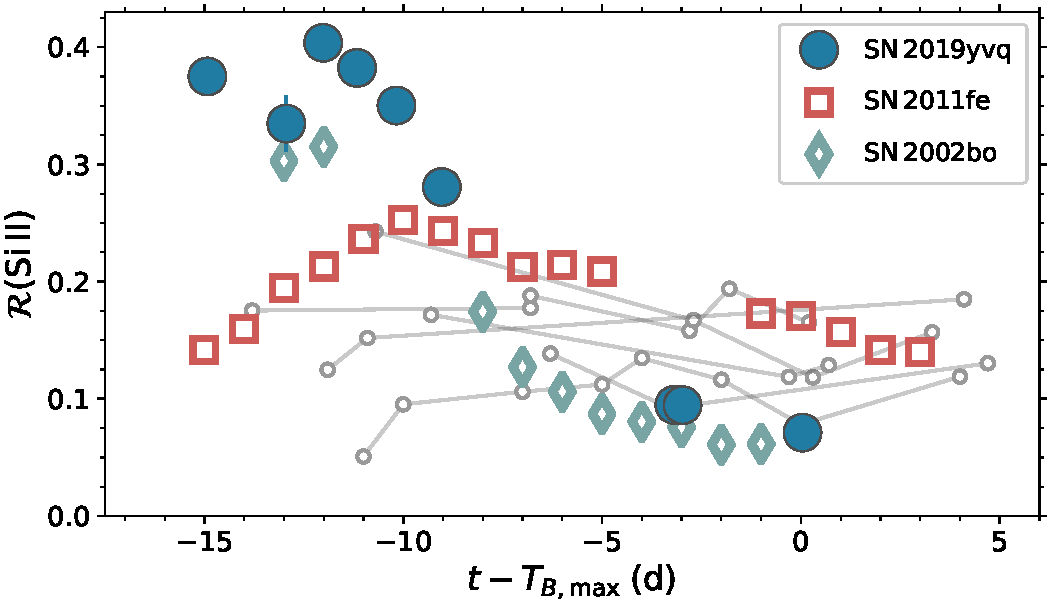
\includegraphics[width=3.35in]{./figures/R_evolution.pdf}
    %
    \caption{Evolution of the ratio of the pEW of \ion{Si}{II} $\lambda$5972
    to \ion{Si}{II} $\lambda$6355, $\mathcal{R}($\ion{Si}{II}$)$, in \sn\
    (large, filled circles). SN\,2002bo \citep[data from][]{Benetti04} and
    SN\,2011fe \citep[data from][]{Pereira13} are also highlighted as open
    diamonds and open squares, respectively. For comparison we also show the
    $\mathcal{R}($\ion{Si}{II}$)$ evolution for 5 PTF SNe\,Ia (10mwb, 10qjq,
    10tce, 10wof, 11hub) with $> 3$ measurements over a duration $> 8$\,d
    (data from \citealt{Maguire14}) and SN\,2017erp \citep[data
    from][]{Brown19} as connected, open circles. \sn\ and SN\,2002bo exhibit
    an unusual inversion in $\mathcal{R}($\ion{Si}{II}$)$ as they evolve
    toward maximum light.}
    %
    \label{fig:r_evo}
\end{figure}

At face value, the $\mathcal{R}($\ion{Si}{II}$)$ evolution in
Figure~\ref{fig:r_evo} suggests that the effective temperature of \sn\
increases significantly as it rises to maximum light. Both the optical colors,
which become bluer in the $\sim$14\,d leading up to \tbmax\ (see
Figure~\ref{fig:colors}), and the \texttt{TARDIS} modeling (see
Table~\ref{tab:tardis}) confirm an increase in temperature over the period in
which $\mathcal{R}($\ion{Si}{II}$)$ decreases. While the UV\,$-$\,optical
colors evolve to the red over the same time period, this is likely due to the
increasing IGE fraction, and hence increased UV blanketing, as the photosphere
recedes (see \S\ref{sec:tardis}), and not a decrease in temperature.

This behavior is similar to, though less extreme than, SN\,2002bo, which
increases in temperature from $\sim$9,500\,K at $-12.9$\,d to $\sim$14,000\,K
at maximum light \citep{Stehle05}. The maximum light temperature of SN\,2002bo
is similar to \citeauthor{Branch06}~Core Normal SNe, such as SN\,2011fe, which
typically have temperatures of $\sim$14,500--15,000\,K at maximum light
\citep{Mazzali14}.

\citet{Benetti04} interpreted these competing effects as the result of
significant \ion{Si}{II} mixing in the ejecta of SN\,2002bo. Mixing or Si
production in the outermost layers of the ejecta would (i) lead to larger
\ion{Si}{II} velocities, (ii) produce \ion{Si}{II} line ratios that indicate
cool temperatures (because there is less radioactive material to heat the
ejecta), before eventually (iii) producing low values of
$\mathcal{R}($\ion{Si}{II}$)$ as the photosphere recedes through the ejecta to
higher temperature regions. This picture is consistent with the
\citet{Stehle05} models of SN\,2002bo. In those models, Si completely
dominates the species at velocities above $\sim$23,000\,\kms, while there is
very little ($\sim$1\%) IGE above a 1.35\,$M_\odot$ in radial mass
coordinates. A similar physical scenario likely explains the changes in
\ion{Si}{II} absorption seen in \sn. Although the temperature change in \sn\
is less dramatic than in SN\,2002bo, this may reflect slight differences in
the ejecta composition as we find \sn\ is consistent with no IGEs in the outer
layers of the SN ejecta.

\subsection{Spectral Comparison}\label{sec:spec_comp}

%%%Comparison to other objects & Si II ratio
In Figure~\ref{fig:spec_comp}, we compare the spectral evolution of \sn\ to
two Broad-Line SNe, SN\,2002bo and SNe\,2010jn, and two Cool SNe, SN\,1986G
and SN\,2004eo \citep{Cristiani92,
Benetti04,Pastorello07,Silverman11,Hachinger13,Maguire14} at four phases,
pre-maximum, maximum, $\sim$1 week post maximum, and $\sim$6 weeks post
maximum. The evolution of \sn\ and SN\,2002bo is remarkably similar at all
phases. The only significant difference between the two is the absorption
trough at $\sim$4800\,\AA\ in the pre- and maximum-light spectra. This
feature, which is typically attributed to a combination of \ion{Fe}{II},
\ion{Fe}{III}, and \ion{Si}{II}, is extremely narrow in \sn. This is in
agreement with the \texttt{TARDIS} modeling results where no Fe is required in
the outer ejecta of \sn\ to match the observed spectra at early times.
SN\,2010jn, which exhibits large \ion{Si}{II} velocities like \sn, shows
weaker IME absorption and stronger IGE absorption than \sn. While the
\citeauthor{Branch06}~Cool SNe\,1986G and 2004eo show lower velocities than
\sn, there is strong agreement in the relative \ion{Si}{II} line strengths of
SN\,1986G and the earliest spectra of \sn.

% The left panel of Figure~\ref{fig:spec_comp} also shows the spectrum of
% SN\,1986G, a \citet{Branch06} Cool SN that is sometimes referred to as
% ``transitional'' given its intermediate properties between normal SNe\,Ia and
% the sub-luminous SN\,1991bg-like population (e.g., \citealt{Pastorello07}).
% The \ion{Si}{II} line ratios, and narrow $\sim$4800\,\AA\ feature in SN\,1986G
% are similar to \sn, confirming the cool nature of the photosphere at this
% early epoch. The $-12.0$\,d spectrum of \sn\ additionally shows a weaker blue
% line in the \ion{S}{II} ``W'' absorption feature at $\sim$5400\,\AA, which is
% also consistent with cool temperatures \citep{Nugent95}.

\begin{figure*}
    \centering
    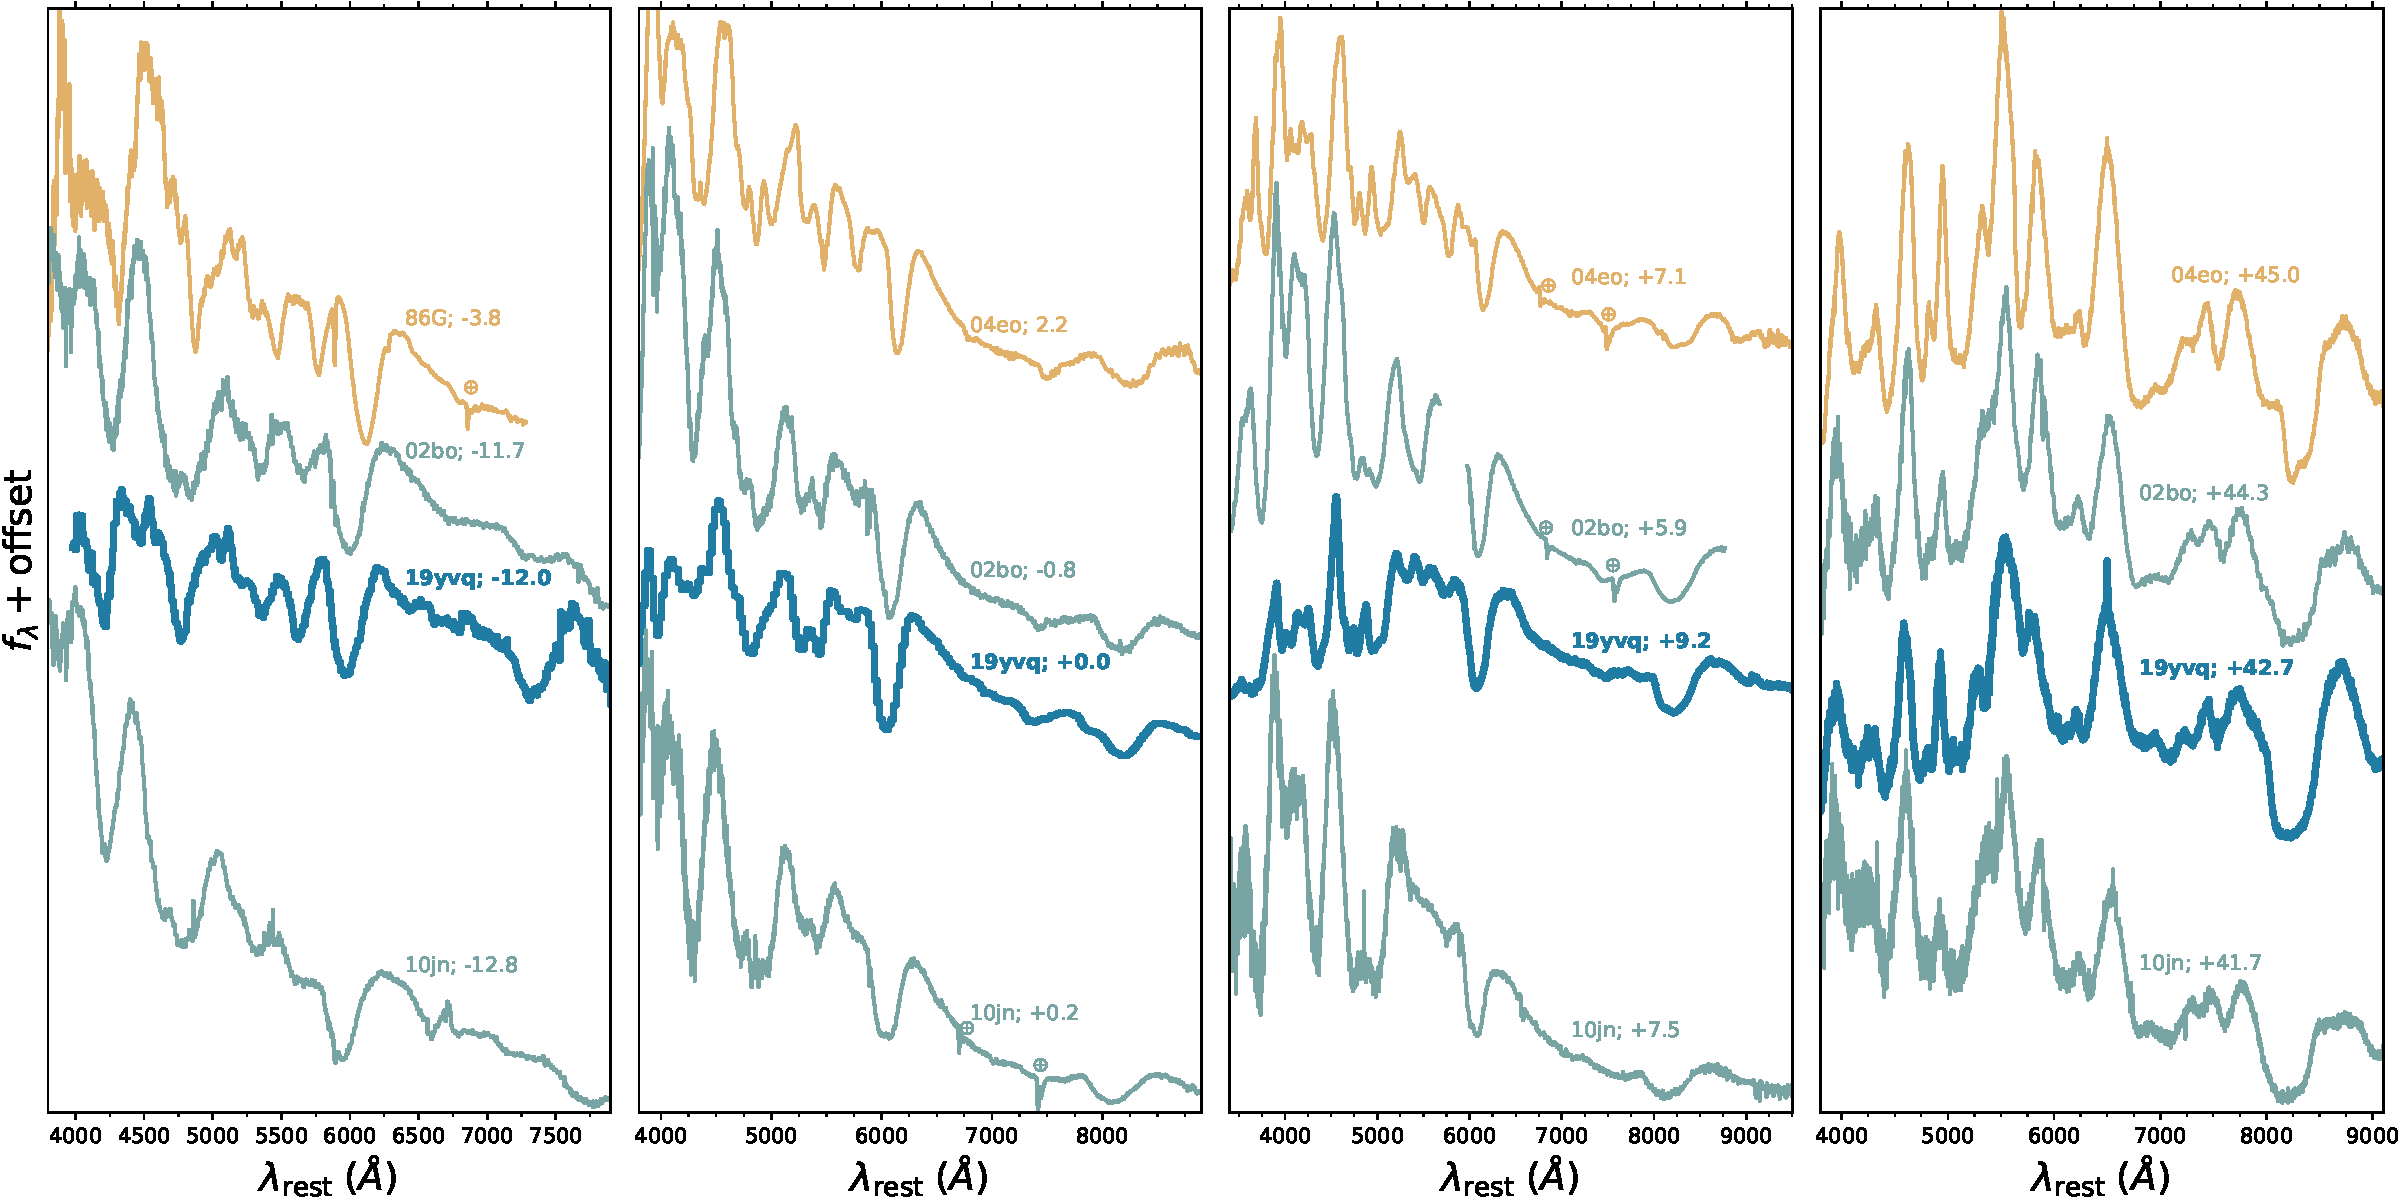
\includegraphics[width=\textwidth]{./figures/spec_comp_extinction.pdf}
    %
    \caption{Spectral comparison of \sn\ to \citeauthor{Branch06}~Broad Line
    and Cool SNe\,Ia. All spectra have been corrected for the total
    line-of-sight extinction with adopted $E(B-V)$ values of 0.9\,mag,
    0.38\,mag, 0.39\,mag, 0.109\,mag, and 0.05\,mag for SNe\,1986G
    \citep{Phillips87}, 2002bo \citep{Stehle05}, 2010jn \citep{Hachinger13},
    2004eo \citep{Pastorello07}, and \sn\ (this work), respectively.
    \textit{Left panel}: pre-maximum spectra showing the similarity of \sn\
    and SN\,2002bo. While the expansion velocities in the Cool SN\,1986G
    spectrum are considerably lower than those in the Broad Line SNe, the
    relative ratios of the \ion{Si}{II} features are similar to \sn.
    \textit{Second panel}: Comparison of \sn\ to the Broad Line SNe\,2002bo
    and SN\,2010jn. These SNe all feature nearly identical maximum-light
    spectra. By this phase, the relative strength of the \ion{Si}{II}
    absorption features is no longer similar to \citet{Branch06} Cool SNe, as
    illustrated by SN\,2004eo. \textit{Third panel}: $\sim$1 week post-maximum
    spectra. \textit{Fourth panel}: Transitional phase spectra. Comparison
    spectra have been downloaded from WISeREP \citep{Yaron12}, with spectra
    for individual SNe from the following sources: SN\,1986G --
    \citet{Cristiani92}, SN\,2002bo -- \citet{Benetti04,Silverman11},
    SN\,2010jn (PTF\,10ygu) -- \citet{Hachinger13,Maguire14}, SN\,2004eo --
    \citet{Pastorello07}.}
    %
    \label{fig:spec_comp}
\end{figure*}

The maximum-light spectra shown in the second panel of
Figure~\ref{fig:spec_comp} reveal a higher temperature for \sn, as the
\ion{Si}{II} $\lambda$5972\,\AA\ absorption has nearly disappeared around
\tbmax\ (see discussion of $\mathcal{R}($\ion{Si}{II}$)$ in \S\ref{sec:SiII}).
This increase in temperature is consistent with the change in optical colors
(Figure~\ref{fig:colors}) and \texttt{TARDIS} spectral modeling
(\S\ref{sec:tardis}). The appearance of \sn, SN\,2002bo, and SN\,2010jn are
all similar at this epoch, with the exception of the 4800\,\AA\ feature
mentioned above. SN\,2004eo has a similar appearance to \sn, though it has
lower velocities and cooler temperatures (as traced by \ion{Si}{II}
$\lambda$5972).

The $+9.2$\,d spectrum of \sn, shown in the third panel of
Figure~\ref{fig:spec_comp}, shows absorption due to IGE. Additional
differences between \sn\ and SN\,2002bo can be seen at this phase. There is
stronger absorption in \sn\ blueward of \ion{Ca}{II} H\&K, and the \ion{S}{II}
``W'' absorption feature is still present in \sn\ and it cannot be identified
in SN\,2002bo or SN\,2010jn. SN\,2004eo maintains an appearance that is
somewhat similar to \sn, though as before, the temperature (as indicated by
\RSiII) is cooler and the velocities lower.

Spectra obtained $\sim$6 weeks after maximum light are shown in the fourth
panel of Figure~\ref{fig:spec_comp}. By this time, as the SNe are
transitioning into a nebular phase, the appearance of each spectrum is similar
modulo some minor differences in the relative line strengths of different
features.

\section{A Physical Explanation for \sn}\label{sec:models}

The most striking feature of \sn\ is the observed UV/optical peak that occurs
shortly after discovery (Figure~\ref{fig:p48}). Any model to explain \sn\ must
account for this highly unusual feature. A UV decline in the early phase of a
SN\,Ia has previously only been observed in a single event, iPTF\,14atg
\citep{Cao15}. Clearly resolved ``bumps'' in the early optical emission of
SNe\,Ia are also rare, having only been seen in a few events: SN\,2014J
\citep{Goobar15}, MUSSES1604D \citep{Jiang17}, SN\,2017cbv
\citep{Hosseinzadeh17} and SN\,2018oh \citep{Shappee19,Dimitriadis19}.

\sn\ features other properties, in addition to an initial peak $\sim$17\,d
prior to \tbmax, that separate it from normal SNe\,Ia. A good model should be
able to explain the properties:
%
\begin{enumerate}
    \item The early UV/optical ``flash'' (Figure~\ref{fig:p48}).
    \item The moderately faint peak in the optical (\S\ref{sec:max_decline}). 
    \item The relatively fast optical decline (\S\ref{sec:max_decline}). 
    \item The red optical colors at all epochs (Figure~\ref{fig:colors}). 
    \item The lack of IGE in the early spectra (\S\ref{sec:tardis}).
    \item The evolution in \RSiII\ (\S\ref{sec:SiII} and Figure~\ref{fig:r_evo}).
    \item The high photospheric velocities (Figure~\ref{fig:vel_evo}).
    % \item The lack of C in the early spectra (\S\ref{sec:tardis}) \todo{check all discussions of Carbon}
\end{enumerate}
%
The moderately faint peak combined with the large \ion{Si}{II} velocity is
particularly rare (see e.g., Figure~11 in \citealt{Polin19}, where \sn\ would
be well isolated from all the other SNe\,Ia). This suggests that \sn\ has a
relatively high kinetic energy despite a relatively low \radni\ yield.

As noted in \S\ref{sec:max_decline}, the photometric evolution of \sn\ is
similar to intermediate 86G-like SNe, however, the spectra feature much weaker
\ion{Si}{II} $\lambda$5972 absorption and larger expansion velocities than
what is seen in 86G-like SNe (see Figure~\ref{fig:spec_comp}). Similarly,
while the spectral appearance and evolution of \sn\ is similar to SN\,2002bo,
and other \citeauthor{Branch06}~Broad Line SNe, the photometric properties are
entirely different. SN\,2002bo features a relatively slow decline
[$\Delta{m}_{15}(B) = 1.13$\,mag] with a clear secondary maximum in the $I$
band \citep{Benetti04}, which stands in contrast to moderately fast decline
[$\Delta{m}_{15}(g) = 1.3$\,mag] and lack of \iztf\ secondary maximum in \sn.

If we otherwise ignore the early flash, several of the remaining features
(2--6) in the list above can be understood if the explosion that gave rise to
\sn\ produced a relatively small amount of \radni\ that is strongly confined
to the inner regions of the SN ejecta. A low \radni\ yield could explain the
underluminous light curve and red colors, while a centrally concentrated IGE
distribution could explain the IME-dominated early spectra, as the IGE would
not have been mixed to these outer layers. Furthermore, with a centrally
compact IGE ejecta composition, the photosphere would transition somewhat
rapidly from \radni-poor to \radni-rich, resulting in a significant change in
the luminosity/temperature of the ejecta along the lines of what we see in the
evolution of \RSiII.

\citet{Magee20} developed a suite of models featuring different \radni\
structures within the SN ejecta. These models were compared to early
observations of SNe\,Ia to see which ones replicate what is observed in
nature. Generally, it is found that centrally concentrated \radni\ models do
not match the early evolution of normal SNe\,Ia \citep{Magee20}. However, when
we model the rise of \sn\ using the models of \citet{Magee20}, we find that
the observations are best matched by compact \radni\ distributions. For this
modeling we have excluded the first two epochs of ZTF observations, as we
consider the mechanism that produces the early UV flash to be different from
the standard \radni\ decay that powers most SNe\,Ia. That the (normal) rising
portion of the \sn\ light curve is best matched by stratified models
strengthens the support for this interpretation. We note, however, that
\citet{Magee20} demonstrate that the time of first detection can dramatically
alter the inferred model properties and it is unclear which epochs (if any)
should be excluded. Nevertheless, a stratified ejecta is also consistent with
our spectroscopic analysis (see \S\ref{sec:tardis}).

On their own, a low-\radni\ yield that is centrally concentrated fails to
explain the blue UV/optical flash seen in \sn. A large number of scenarios
have been proposed to explain early ``bumps'' or ``flashes'' in SNe\,Ia light
curves, including: interaction between the SN ejecta and the WD binary
companion \citep{Kasen10a}, interaction between the SN ejecta and
circumstellar material (e.g., \citealt{Dessart14,Piro16,Levanon17}), shock
cooling following the shock breakout from the surface of the WD (e.g.,
\citealt{Piro10,Rabinak11}), double-detonation explosions (e.g.,
\citealt{Noebauer17,Polin19}), and extended clumps of \radni\ in the SN ejecta
(e.g., \citealt{Shappee19,Dimitriadis19}). We discuss these models and their
ability to replicate observations of \sn\ below.\footnote{We do not discuss
shock breakout models as our initial detection of \sn\ occurred at $M_g
\approx -16.3$\,mag. A progenitor radius of $\sim$10$\,R_\odot$ is needed to
explain such a high luminosity \citep{Piro10,Rabinak11}, which we consider
implausible for a WD.}

\subsection{Companion Interaction}\label{sec:companion_interaction}

For SD progenitors of SNe\,Ia, the SN ejecta will shock on the surface of the
non-degenerate companion giving rise to a short-lived transient in the days
after explosion. \citet{Kasen10a} provided models for the appearance of this
interaction, which is primarily dependent upon the binary separation of the
system (assuming Roche lobe overflow for the non-degenerate companion). The
observed emission following the ejecta-companion collision is dependent upon
the orientation of the system at the time of explosion relative to the line of
sight \citep{Kasen10a}.

An analytic formulation for the luminosity and effective temperature of the
emission from the companion shock is given in Equations~22 and 25 in
\citet{Kasen10a}. \citet{Brown12} provide an analytic function to approximate
the fractional decrease in the observed flux as a function of the orientation
of the system. We combine equations from \citet{Kasen10a} and \citet{Brown12}
to model the early emission from \sn\ as ejecta-companion collision. We assume
the interaction emits as a blackbody, and that the electon scattering opacity
$\kappa_e = 0.2$\,cm$^{2}$\,g$^{-1}$ (as in \citealt{Kasen10a}). Assuming
$z_\mathrm{SN} = 0.0094$, $E(B-V)_\mathrm{MW} = 0.018$\,mag, and
$E(B-V)_\mathrm{host} = 0.032$\,mag, we compare observed flux measurements
with those predicted by the \citet{Kasen10a} model in epochs with MJD$\,<
58849.2$ (i.e., the first $\sim$2.5\,d after discovery when emission from the
companion interaction is significantly brighter than the luminosity due to
radioactive decay).\footnote{Given that \sn\ is an unusual SN, we make no
assumptions about the ``normal'' SN emission due to radioactive decay of
\radni. The companion-interaction model should therefore
\textit{underestimate} the observed flux as there will be a growing
contribution due to radioactive decay with time.} The model parameters,
including: the companion separation, $a$, the mass of the ejecta,
$M_\mathrm{ej}$, the velocity of the ejecta, $v_\mathrm{ej}$, the angle
between the observer, the SN, and the companion, $\theta$, and the time of
explosion, $t_\mathrm{exp}$ are constrained via a Gaussian likelihood and flat
priors (see Table~\ref{tab:priors}) using an affine-invariant
\citep{Goodman10} Markov Chain Monte Carlo (MCMC) ensemble sampler
\citep{Foreman-Mackey13}.

\begin{figure}
    \centering
    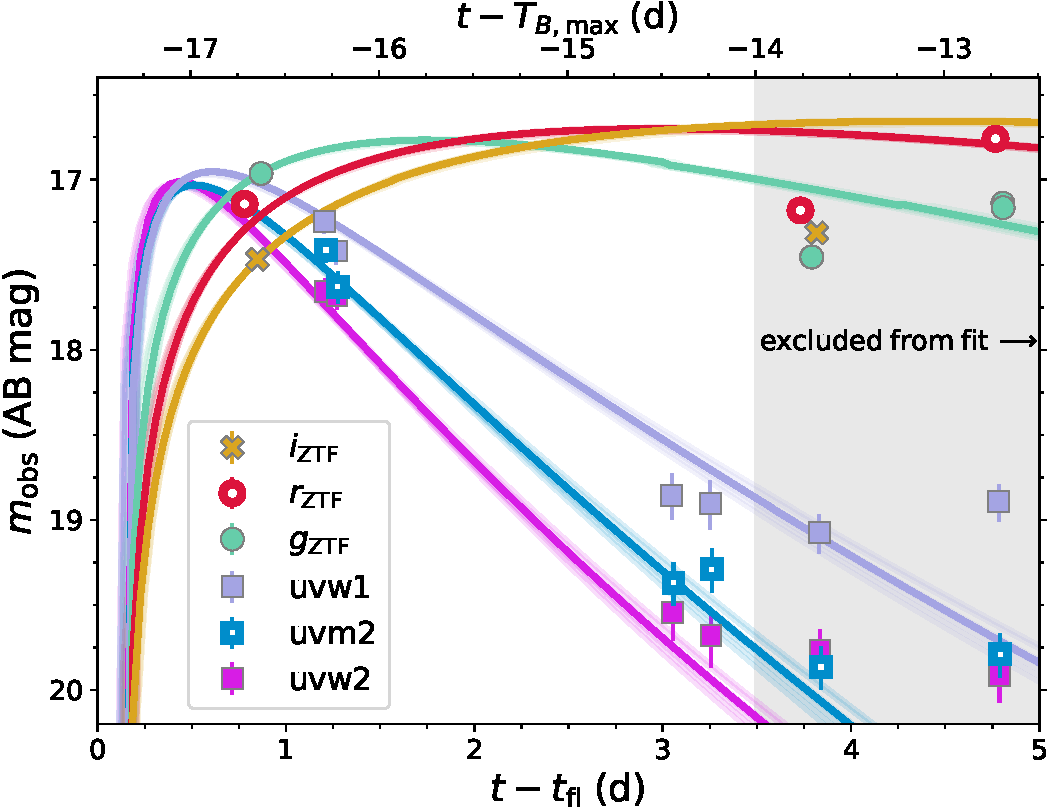
\includegraphics[width=3.35in]{./figures/sn_companion_models.pdf}
    %
    \caption{SN ejecta-companion interaction models compared with the
    UV/optical observations of \sn. Observation symbols are the same as
    Figure~\ref{fig:p48} (solid magenta squares show \textit{Swift} $uvw2$
    observations that are not shown in Figure~\ref{fig:p48}). Solid lines show
    companion interaction model predictions in each filter (the lines have the
    same colors as the corresponding symbols for each passband). The maximum a
    posteriori model is shown via the single bold lines, while other random
    draws from the posterior are shown as thin transparent lines. The shaded
    area shows observations that are excluded from the model fit. The
    overprediction of the optical flux $\sim$13.7\,d prior to \tbmax\ suggests
    that companion interaction does not explain the early flash in \sn\ (see
    text).}
    %
    \label{fig:companion}
\end{figure}

The results of this procedure are shown in Figure~\ref{fig:companion}, where
it is clear that the model presented in \citet{Kasen10a} does an adequate job
of explaining the early UV/optical emission from \sn. We find marginalized
posterior values of $a = 9.1 \pm 0.7 \times 10^{11}$\,cm, $M_\mathrm{ej} = 1.0
\pm 0.3\,M_\odot$, $v_\mathrm{ej} = 2.2 \pm^{0.5}_{0.3} \times 10^{4}$\,\kms,
$\theta = 34 \pm^{28}_{24} \deg$, and $t_\mathrm{exp}(\mathrm{MJD}) = 58845.83
\pm 0.05$ (all uncertainties are 68\% credible regions). Examination of a
corner plot of the posterior samples shows that $M_\mathrm{ej}$ is largely
unconstrained, while $v_\mathrm{ej}$ is degenerate with $\theta$ and $a$ is
degenerate with $t_\mathrm{exp}$. 

While the interaction models roughly approximate the SN emission in the
$\sim$3\,d after explosion, they significantly \textit{overestimate} the flux
immediately after the fitting window as shown in Figure~\ref{fig:companion}.
This problem is exacerbated by the fact that the models do not include
emission associated with radioactive decay, meaning the true discrepancy
between what is predicted and what is observed is even larger than what is
shown in Figure~\ref{fig:companion}. If we extend the fitting window to
include the optical observations obtained $\sim$13.75\,d before \tbmax, the
interaction models still overpredict the optical flux at this epoch. This
overprediction of the optical flux poses a challenge for the companion
interaction scenario; an inability to simultaneously match both UV and optical
observations has been noted for other SNe\,Ia with early bumps or linear rises
\citep{Hosseinzadeh17,Miller18}.

For this reason, we do not favor the ejecta-companion interaction
interpretation for \sn. \citet{Kasen10a} notes several assumptions and
approximations in the derivation of the equations used to estimate the
emission from the companion shock. It is possible that the inclusion of more
detailed physics, or additional complexity in the analytic formulation of the
models,\footnote{For example, \citet{Kasen10a} points out that the derived
equation for the luminosity of the shock interaction does not account for the
advected luminosity that would be seen in the observer frame.} could better
reconcile companion interaction models with \sn. Such improvements are beyond
the scope of this paper, leading us to explore other explanations for the
early flash.

\subsection{Ni Clumps in the SN Ejecta}

SN\,2018oh was observed with an exquisite 30\,min cadence by the
\textit{Kepler} spacecraft and showed a clearly delineated linear rise in flux
followed by a ``standard'' $t^2$ power-law $\sim$4\,d after \tfl. Models with
extended clumps of \radni\ just below the WD surface have been proposed as a
possible explanation for the initial linear rise in SN\,2018oh
\citep{Shappee19,Dimitriadis19}. The models considered in \citet{Shappee19}
and \citet{Dimitriadis19}, which build on the work of \citet{Piro16}, only
cover the first $\sim$10\,d after explosion and assume relatively simple grey
opacities. To further investigate this possibility, \citet{Magee20a} recently
performed more detailed radiative transfer calculations for SNe\,Ia with
extended clumps of \radni. They then compared these models to SN\,2018oh and
SN\,2017cbv, another event with a clearly resolved bump in the early light
curve \citep{Hosseinzadeh17}.

\begin{figure}
    \centering
    \includegraphics[width=3.35in]{./figures/clump_spec.pdf}
    %
    \caption{Spectroscopic comparison between \sn\ and our model with a clump
    of \radni\ in the outer ejecta. Observed spectra of \sn\ are shown in
    blue, with phases marked relative to \tbmax, whereas the model spectra are
    shown in dark grey, with phases marked relative to the modelled time of
    explosion. For the comparison we have adopted a model explosion time
    $t_\mathrm{exp} = t_\mathrm{fl} - 1.67$\,d. The modelled spectra have been
    smoothed with a Savitzky-Golay filter \citep{Savitzky64}. While an
    extended clump of \radni\ in the SN ejecta can recreate the early optical
    flash, it leads to strong blanketing in the blue portion of the optical
    that is not observed around maximum light in \sn. }
    %
    \label{fig:Ni_bullet}
\end{figure}

For \sn\ we follow the procedure in \citet{Magee20a} to model the early flash
and rise of the SN. Briefly, we exclude the first two epochs of optical
detections in ZTF, and identify the best-fit model to the later evolution of
the SN from the grid of models created in \citet{Magee20}. Following the
generation of this ``baseline'' model, we add clumps of \radni\ to the outer
layers of the SN ejecta, and perform full radiative transfer calculations
using \texttt{TURTLS} \citep{Magee18}. We find that a model with a
0.02~$M_{\rm{\odot}}$ clump of \radni\ adequately matches the early optical
evolution of \sn. As found in \citet{Magee20a}, however, such models face a
significant challenge in that the extended clump of \radni\ dramatically
alters the appearance of the SN at maximum light. Figure~\ref{fig:Ni_bullet}
shows a comparison of the observed spectra with our calculated models. The Ni
clump models feature strong blanketing in the blue-optical, which is simply
not present in the observed spectra of \sn. We therefore conclude that Ni
clumps cannot explain the early flash seen in \sn.

\subsection{Double-Detonation Models}

WDs that accrete a thin shell of He can explode via a ``double detonation''
whereby explosive burning in the He shell drives a shock into the C/O core of
the WD. This shock can ignite explosive C burning and a detonation that
disrupts the entire star (e.g., \citealt{Nomoto82,Nomoto82a,Woosley94}). Such
explosions are even possible in C/O WDs that are well below the Chandrasekhar
mass (see \citealt{Fink07, Fink10} and references therein).

Recent models of double-detonation explosions presented in \citet{Polin19}
show that such explosions can replicate several of the peculiar properties of
\sn, including: the early UV/optical flash, a blue to red to blue color
transition, the moderately faint optical peak, red colors at maximum, and a
lack of IGE in the early spectra.

The appearance of double-detonation SNe is effectively determined by two
properties: the mass of the C/O core and the mass of the He shell. The total
mass of the system determines the central density of the WD and thus the
amount of synthesized \radni. The \radni\ mass directly controls both the peak
luminosity and the kinetic energy of the explosion. High mass WDs ($\gtrsim
1.1\,M_\odot$) create enough \radni\ ($M_\mathrm{Ni} \gtrsim 0.5\,M_\odot$) to
produce large ($\gtrsim 1$4,000\,\kms) photospheric velocities and reach
normal brightness for a SN\,Ia, while low mass WDs ($\lesssim 0.9\,M_\odot$)
exhibit slower photospheric velocities ($\lesssim 1$0,000\,\kms) and produce
less \radni, therefore peaking at fainter luminosities \citep{Polin19}. That
we see both a high \ion{Si}{II} velocity and a low peak luminosity in \sn\
presents a challenge for the \citet{Polin19} double-detonation models.
Furthermore, thick He shells ($M_\mathrm{He} \gtrsim 0.05\,M_\odot$) produce
more pronounced UV/optical flashes shortly after explosion, particularly in
conjunction with lower mass WDs, while thin He shells ($M_\mathrm{He} \lesssim
0.02\,M_\odot$) produce a more extreme color inversion in the days after
explosion.

We have attempted to model the evolution of \sn\ as a double-detonation
explosion, following the procedure in \citet{Polin19}. We have specifically
focused on matching the photometric evolution (as noted above no models create
high-velocity ejecta and underluminous optical peaks), with particular
attention to the colors during the early flash and at maximum light. We find
that a model with $M_\mathrm{C/O} = 0.92\,M_\odot$ C/O core and a
$M_\mathrm{He} = 0.04\,M_\odot$ He shell best match \sn, as shown in
Figure~\ref{fig:double_det}.

\begin{figure*}
    \centering
    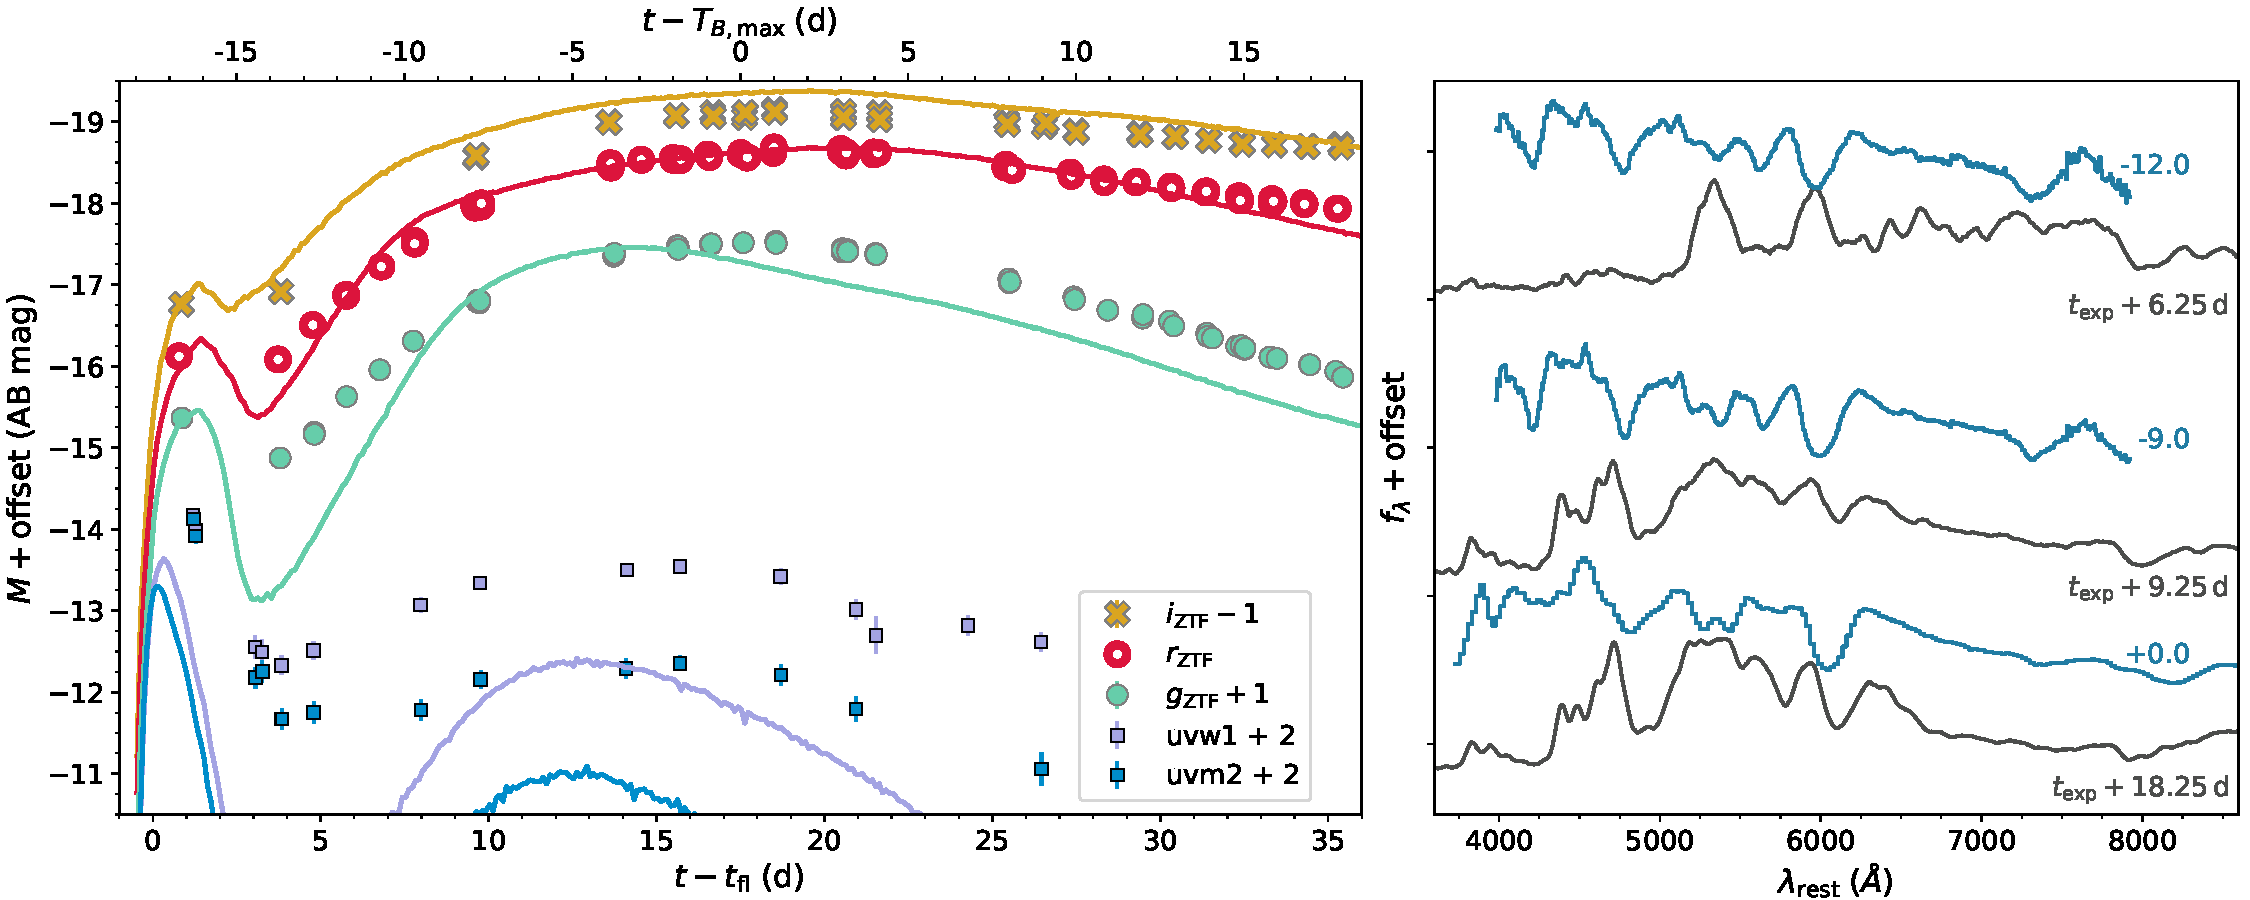
\includegraphics[width=\textwidth]{./figures/double_det.pdf}
    %
    \caption{Comparison of \sn\ to a dobule-detonation model with a C/O core
    mass $M_\mathrm{C/O} = 0.92\,M_\odot$ and He shell mass $M_\mathrm{He} =
    0.04\,M_\odot$ (i.e., $M_\mathrm{WD} = 0.96\,M_\odot$). For the comparison
    we have adopted a model explosion time $t_\mathrm{exp} = t_\mathrm{fl} -
    0.72$\,d. \textit{Left}: Photometric comparison between \sn\ and the
    model. Symbols are the same as Figure~\ref{fig:p48}. The double-detonation
    model provides a good match to the \rztf\ evolution, though the flux in
    the \gztf\ and \iztf\ bands is under- and over-predicted, respectively.
    The UV emission is also underestimated by the double-detonation model.
    \textit{Right}: Spectroscopic comparison between \sn\ and the model.
    Observed spectra of \sn\ are shown in blue, with phases marked relative to
    \tbmax, whereas the model spectra are shown in dark grey, with phases
    marked relative to the modelled time of explosion. The modelled spectra
    have been smoothed with a Savitzky-Golay filter \citep{Savitzky64}. The
    photospheric velocity in the double-detonation model is lower than what is
    observed in \sn, and the models feature more absorption and blanketing in
    the blue portion of the optical than what is observed. }
    %
    \label{fig:double_det}
\end{figure*}

While this model adequately matches the evolution of \sn\ in the \rztf\
filter, the predictions in the \gztf\ and \iztf\ bands do not match what is
observed. We show for the first time that there is an expected UV flash
associated with these double-detonation models, however, our best fit model
underestimates the flux that was observed in the UV.

Synthesized spectra from our double-detonation model exhibit features that are
not seen in \sn. The model spectra are dominated by \ion{Si}{II} absorption,
and show high-velocity absorption due to \ion{O}{I} and \ion{Ca}{II}, similar
to \sn. For our best-fit model, however, the \ion{Si}{II} velocities are too
slow, the \ion{Si}{II} $\lambda$5972 absorption is too strong, and the
\ion{S}{II} absorption too weak. Nuclear burning in the He shell creates heavy
elements in the outermost ejecta of double-detonation explosions, leading to
deep \ion{Ti}{II} troughs and other blanketing in the blue-optical. Our model
exhibits a strong \ion{Ti}{II} absorption trough blueward of $\sim$4400\,\AA\
(see the $t_\mathrm{exp} + 9.25$\,d spectrum in Figure~\ref{fig:double_det}).
As was the case for models with extended clumps of \radni, the lack of such
absorption in \sn\ poses a challenge for the double-detonation model.

With observations that probe a previously unexplored phase in the evolution of
such explosions, \sn\ provides an opportunity to determine where the
double-detonation models must improve. It is possible that such improvements
could lead to better agreement with \sn. For instance, the nuclear reaction
networks and 1D models in \citet{Polin19} always burn the He shells to nuclear
statistical equilibrium. It is not unreasonable to think that 2D or 3D models,
with a more sophisticated nuclear reaction network, would create more IMEs and
less IGEs in the He shell, and that the ratio of the two created in the shell
could be highly dependent upon the line of sight. This could explain the lack
of IGEs and strong \ion{Si}{II} absorption seen in the early spectra, while
less IGEs in the outer layers would also reduce some of the line blanketing
seen around maximum light. This would lead to less reprocessing of blue
photons, perhaps creating better agreement between the models and photometry,
particularly in the \gztf\ band. The velocity discrepancy could also
potentially be explained as a line-of-sight effect. If the ignition of the WD
occurred off center, then the ejecta aligned with the site of the initial He
ignition may receive a boost in velocity. The discrepancies in the UV are less
worrisome. While we show a qualitative UV flash, the magnitude of this flash
will be highly sensitive to the precise temperature and composition in the
very outer most ejecta, and thus any of the changes discussed above could
easily boost the model flux in the UV.

\subsection{Violent Mergers and Circumstellar
Interaction}\label{sec:merger_csm}

\citet{Piro16} show that circumstellar material in the vicinity of a WD at the
time of explosion can give rise to an early flash or bump in the SN\,Ia light
curve. Using a 1D toy model, with an assumed circumstellar density profile
$\propto r^{-3}$ and grey opacities, \citet{Piro16} find that the peak of the
early emission is roughly proportional to the extent of the circumstellar
material, while the duration of the flash is proportional to the square root
of the circumstellar mass. While the brightest model from \citet{Piro16} has a
flash brightness that peaks at $M_V \approx -15$\,mag, circumstellar material
that extends beyond $\sim$10$^{12}$\,cm could give rise to a flash that peaks
at $M_g \lesssim -16.4$\,mag, as is observed in \sn.

There are few proposed WD explosion models that produce dense circumstellar
material in the vicinity of the WD at the time of explosion. A noteable
exception is the violent merger, so called because the thermonuclear explosion
happens while the merger is still ongoing, of two C/O WDs
\citep{Pakmor10,Pakmor11,Pakmor12}. DD mergers should produce a wide variety
of circumstellar configurations depending on the initial parameters of the
inspiralling binary, which would, in turn, produce different signals shortly
after explosion (e.g., \citealt{Raskin13,Levanon19}).\footnote{Indeed, the
large number of potential configurations makes it very difficult to rule out
or select any specific circumstellar interaction scenario.}

Given the vast parameter space populated by different circumstellar
configurations, we are going to proceed under the (potentially poor)
assumption that such interaction could reproduce the UV/optical flash seen in
\sn. Following this assumption, a relevant question is -- can violent mergers
reproduce the properties of \sn\ in the days before and weeks after \tbmax?

In \citet{Kromer16}, the violent merger of two C/O WDs with masses of 0.9 and
0.76\,$M_\odot$ was simulated to recreate the rise and maximum-light
properties of iPTF\,14atg, the other SN\,Ia to show an early UV flash. A
comparison of the low-metallicity model from \citet{Kromer16}, which was tuned
for iPTF\,14atg, \textit{and not \sn}, is shown in
Figure~\ref{fig:violent_merger}. The \citeauthor{Kromer16}~model was not
designed to fit the early UV flash in iPTF\,14atg.

\begin{figure*}
    \centering
    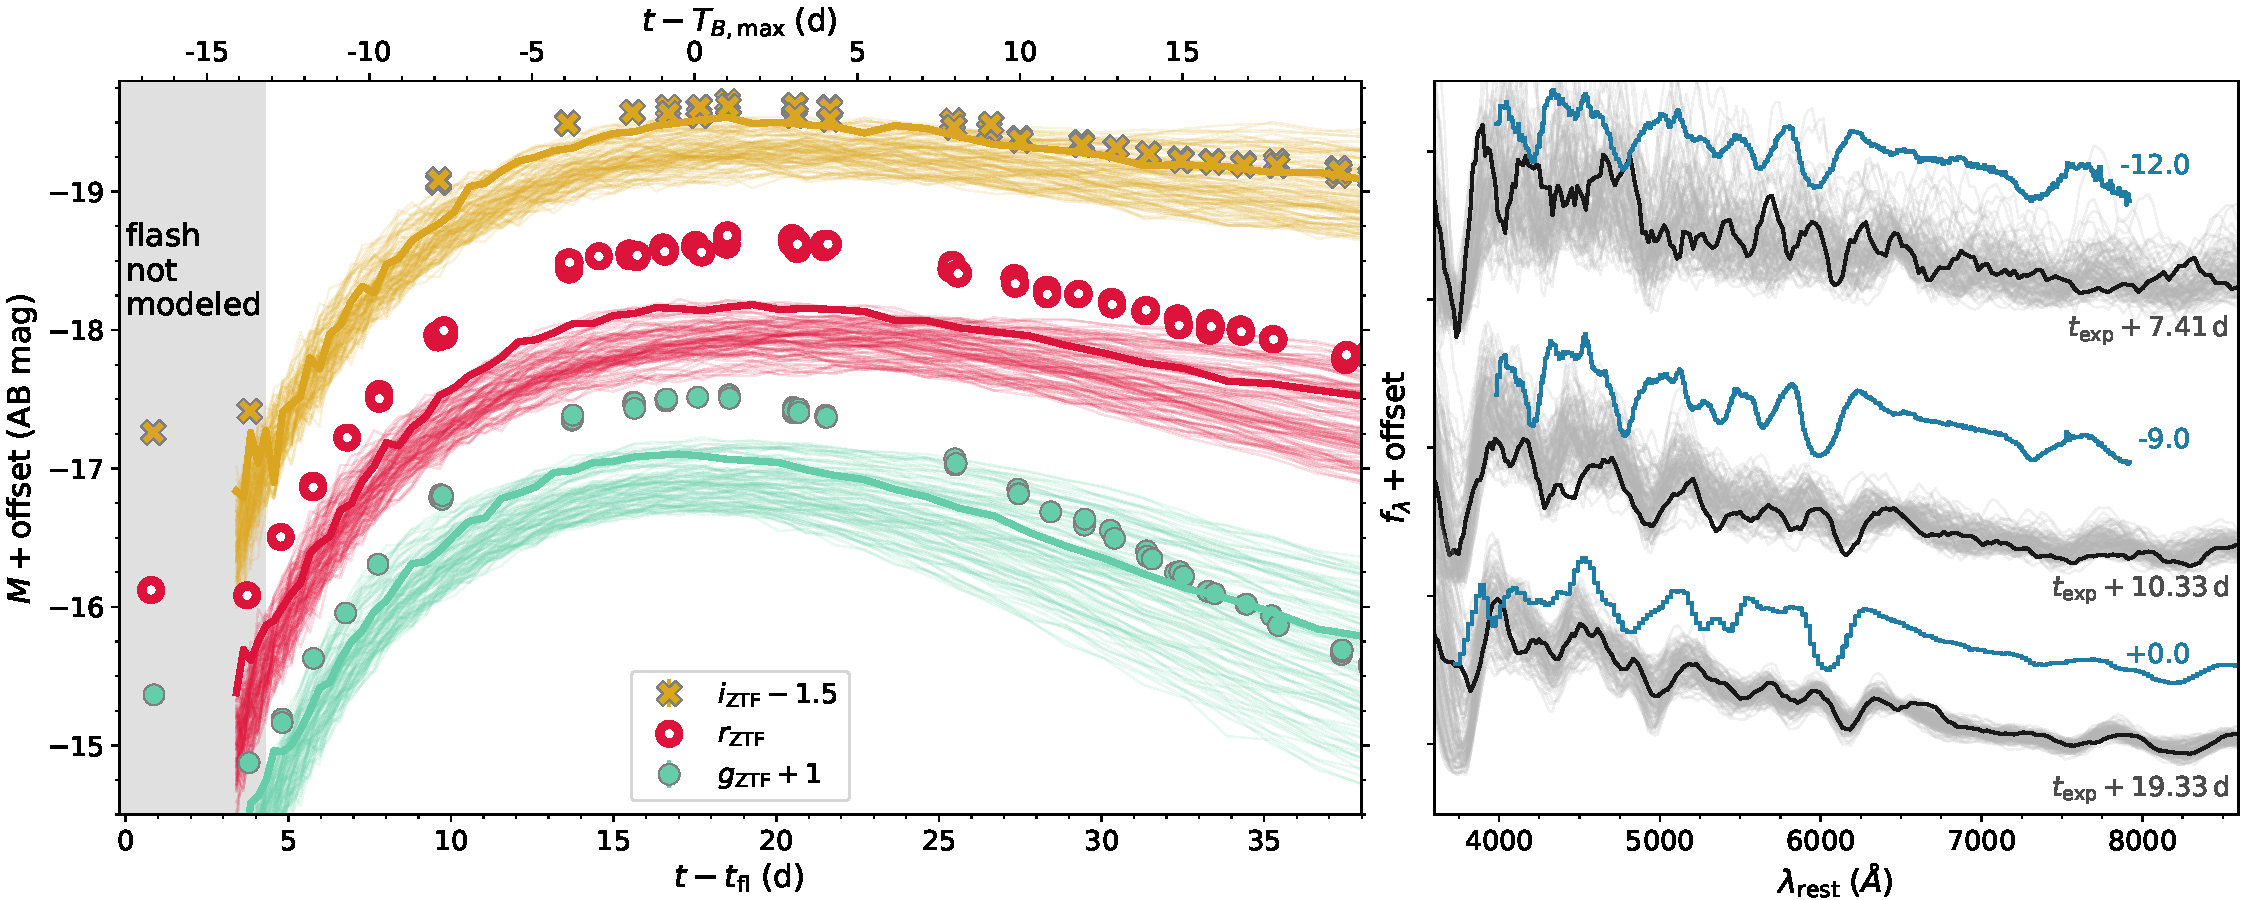
\includegraphics[width=\textwidth]{./figures/violent_merger.pdf}
    %
    \caption{Comparison of \sn\ to the low metallicity ($Z = 0.01 Z_\odot$)
    violent merger model of a 0.9\,$M_\odot$ WD and 0.76\,$M_\odot$ WD from
    \citet{Kromer16}. This model was tuned to match iPTF\,14atg, which is why
    the model significantly underestimates the brightness of \sn. For the
    comparison we have adopted a model explosion time $t_\mathrm{exp} =
    t_\mathrm{fl} - 1.92$\,d. Thin lines represent one of 25 sightlines, while
    the bold lines represent a single sightline for illustrative purposes.
    \textit{Left}: Photometric comparison between \sn\ and the model. Symbols
    are the same as Figure~\ref{fig:p48}. Despite the underestimated optical
    flux, the qualitative behavior of the violent merger model, including red
    \gztf$ - $\rztf\ colors at peak and a lack of secondary maximum in the
    \iztf-band do match \sn. \textit{Right}: Spectroscopic comparison between
    \sn\ and the violent merger model. Observed spectra of \sn\ are shown in
    blue, with phases marked relative to \tbmax, whereas the model spectra are
    shown as thin grey lines. The thick black line highlights a specific
    viewing angle. The modelled spectra have been smoothed with a
    Savitzky-Golay filter \citep{Savitzky64}. The photospheric velocity in the
    violent merger model features lower velocities than \sn, while the
    strength of the the IME absorption is weaker in the models than what is
    observed.}
    %
    \label{fig:violent_merger}
\end{figure*}

The photometric evolution of this violent merger model qualitatively matches
\sn: (i) a moderately faint peak in the optical ($-17.6\,\mathrm{mag} \gtrsim
M_g \gtrsim -18.2$\,mag, depending on the viewing angle), (ii) red $g - r$
colors at peak, and (iii) a lack of a secondary maxmium in the $i$-band.
Furthermore, the spectra lack significant IGE absorption in the days after
explosion (right panel of Figure~\ref{fig:violent_merger}), as is observed in
\sn. A critical difference between \sn\ and violent merger models, is that the
merger models tend to produce relatively low expansion velocities (e.g.,
\citealt{Pakmor10,Kromer13a,Kromer16}). Indeed, this is one of the stark
differences between \sn\ and iPTF\,14atg, as iPTF\,14atg had a \ion{Si}{II}
$\lambda$6355 absorption velocity of $\sim$7,500\,\kms\ at peak, or roughly
half that observed in \sn. It is also clear from
Figure~\ref{fig:violent_merger} that the violent merger model from
\citet{Kromer16} exhibits weaker IME absorption than what is seen in \sn.

It is clear that additional modeling, likely of a different WD binary
configuration, is needed to better match \sn. For example, it is known that a
higher mass primary WD can produce more \radni, and hence a brighter optical
peak \citep[e.g.,][]{Pakmor12}, which would be more in line with \sn. If, at
the same time, the mass of the secondary were slightly decreased, then the
kinetic energy of the ejecta would increase, perhaps bringing the model
velocity of \ion{Si}{II} and other IMEs in line with \sn. It would also be
beneficial to track the unbound material following the DD merger, to see if
the collision between this material and the SN ejecta can replicate the early
UV/optical flash seen in \sn. If this feature can readily be recreated, it is
possible that a violent merger is responsible for \sn.

% \section{Rate of Thick He Shell Double Detonation Events}\label{sec:rates}
%
% \textbf{This may not actually be a thick shell}
%
% \aam{Use rough numbers from CLU and simple binomial calculation}

\section{Discussion and Conclusion}\label{sec:conclusions}

We have presented observations of the spectacular \sn, the second ever SN\,Ia
to exhibit a clear UV/optical flash in its early evolution. Despite this
dazzling, declarative display announcing \sn\ as a unique event among the
thousands of SNe\,Ia that have previously been cataloged, we find that \sn\
would be considered unusual even if the early flash had been missed.

The photometric evolution of \sn\ resembles that of the intermediate 86G-like
subclass of SNe\,Ia. With a moderately faint peak optical brightness ($M_g
\approx -18.5$\,mag), relatively fast decline [$\Delta m_{15}(g) = 1.3$\,mag],
and lack of a secondary maximum in the \iztf\ filter, \sn\ is clearly
distinguished photometrically from normal SNe\,Ia. These photometric
properties typically correspond to \citeauthor{Branch06}\ Cool SNe, yet the
spectroscopic evolution of \sn\ does match such events. \sn\ is a
\citeauthor{Branch06}\ Broad Line SN, with relatively weak \ion{Si}{II}
$\lambda$5972 absorption and large photospheric velocities. Furthermore, our
\texttt{TARDIS} models show little to no IGE present in the outer layers of
the SN ejecta, which further isolates \sn, even relative to other
\citeauthor{Branch06}\ Broad Line SNe. The fact that \sn\ exhibits
high-velocity \ion{Si}{II} $\lambda$6355 absorption and an underluminous peak
sets it apart from other SNe\,Ia.

We have found that building a consistent physical model to explain all of the
observed properties of \sn\ is challenging. Most models either replicate the
early flash but fail to reproduce the observed behavior around maximum light,
or vice versa.

We have examined four models in detail to try and explain the dramatic early
UV/optical peak in \sn, including: the collision of the SN ejecta with a
nondegenerate companion (e.g., \citealt{Kasen10a}), extended clumps of \radni\
in the outer layers of the SN ejecta \citep[e.g.,][]{Magee20a}, the double-detonation explosion of a sub-Chandrasekhar mass WD \citep[e.g.,][]{Polin19},
and the violent merger of two sub-Chandrasekhar mass WDs
\citep[e.g.,][]{Kromer16}.

The SN ejecta-companion models, which can easily replicate the early UV flash
from \sn, simultaneously over-predict the optical flux at similar epochs.
Models with extended clumps of \radni\ produce significant blanketing in the
blue optical. We therefore favor either a double-detonation explosion or a
(violent) merger of two WDs as the origin of \sn. These models are not without
their own shortcomings when it comes to matching the observations. While the
double-detonation model produces an early flash and \rztf\ evolution that
provides a good match to \sn, it too produces blanketing that is too strong in
the blue optical and features photospheric velocities that are much lower than
what is observed. The specific WD merger model from \citet{Kromer16} that we
compare to \sn\ does a poor job of replicating the observations. Many of the
qualitative features match, however, so it is not unreasonable to think that
with some tuning (e.g., higher mass WDs) that the merger model could better
reflect what is observed in \sn.

Nebular spectra of \sn\ will play a crucial role in disambiguating between
these various scenarios. If the ejecta have collided with a nondegenerate
companion, then they will have stripped some surface material from the
companion, which will be revealed via narrow Balmer lines in the nebular phase
\citep[e.g.,][]{Wheeler75}. Alternatively, \citet{Polin19a} recently showed
that low mass ($M_\mathrm{WD} \lesssim 1.0\,M_\odot$) double-detonation
explosions do not create a significant amount of IGEs in their core. This
relative lack of IGEs means that [\ion{Ca}{II}] provides the best pathway for
the ejecta to cool, and as a result strong [\ion{Ca}{II}]
$\lambda\lambda$7291, 7324 emission is expected in the nebular phase. Finally,
violent mergers are expected to exhibit narrow [\ion{O}{I}]
$\lambda\lambda$6300, 6364 emission in their nebular spectra, as unburned O
from the disrupted WD is present at low velocities in the central ejecta
\citep{Taubenberger13,Kromer16}. Each of these predictions are unique to the
scenarios discussed here.

The critical challenge moving forward in understanding \sn-like events is the
rapid acquisition of \textit{Swift} UV observations shortly after explosion.
ZTF, and other similar surveys (ATLAS, ASAS-SN), have demonstrated the ability
to routinely find extremely young SNe\,Ia. Following this the challenge is to
(i) recognize these events as likely SNe\,Ia \textit{at the epoch of
discovery} (i.e., without a significant delay to obtain a spectroscopic
classifcation) and (ii) promptly obtain \textit{Swift} photometry. Only after
these UV observations become as routine as the discoveries themselves will we
be able to statistically answer questions about the nature of SN\,Ia
progenitors. \todo{as is always the case - the last paragraph I've written
sucks}


\acknowledgements

A.A.M.~is funded by the Large Synoptic Survey Telescope Corporation, the
Brinson Foundation, and the Moore Foundation in support of the LSSTC Data
Science Fellowship Program; he also receives support as a CIERA Fellow by the
CIERA Postdoctoral Fellowship Program (Center for Interdisciplinary
Exploration and Research in Astrophysics, Northwestern University).

C.F.~gratefully acknowledges support of his research by the Heising-Simons
Foundation (\#2018-0907).

This work was supported by TCHPC (Research IT, Trinity College Dublin).
Calculations were performed on the Kelvin cluster maintained by the Trinity
Centre for High Performance Computing. This cluster was funded through grants
from the Higher Education Authority, through its PRTLI program.

This work was supported by the GROWTH project funded by the National Science
Foundation under Grant No 1545949.

This work is based on observations obtained with the Samuel Oschin Telescope
48-inch and the 60-inch Telescope at the Palomar Observatory as part of the
Zwicky Transient Facility project. ZTF is supported by the National Science
Foundation under Grant No. AST-1440341 and a collaboration including Caltech,
IPAC, the Weizmann Institute for Science, the Oskar Klein Center at Stockholm
University, the University of Maryland, the University of Washington,
Deutsches Elektronen-Synchrotron and Humboldt University, Los Alamos National
Laboratories, the TANGO Consortium of Taiwan, the University of Wisconsin at
Milwaukee, and Lawrence Berkeley National Laboratories. Operations are
conducted by COO, IPAC, and UW.

This research made use of \texttt{TARDIS}, a community-developed software
package for spectral synthesis in SNe \citep{Kerzendorf14}. The development of
\texttt{TARDIS} received support from the Google Summer of Code initiative and
from ESA's Summer of Code in Space program. \texttt{TARDIS} makes extensive
use of \texttt{Astropy} and \texttt{PyNE}.

MMT Observatory access was supported by Northwestern University and the
Center for Interdisciplinary Exploration and Research in Astrophysics (CIERA).

Partly based on observations made with the Nordic Optical Telescope, operated
at the Observatorio del Roque de los Muchachos, La Palma, Spain, of the
Instituto de Astrof\'isica de Canarias.

This work made use of data supplied by the UK \textit{Swift} Science Data
Centre at the University of Leicester.

\software{\texttt{astropy} \citep{Astropy-Collaboration13}, 
          \texttt{corner} \citep{Foreman-Mackey16},
          \texttt{emcee} \citep{Foreman-Mackey13},
          \texttt{FRODOSpec L2 pipeline} \citep{Barnsley12},
          \texttt{LPipe} \citep{Perley19},
          \texttt{matplotlib} \citep{Hunter07}, 
          \texttt{pandas} \citep{McKinney10},
          \texttt{pyraf-dbsp} \citep{Bellm16b},
          \texttt{pysedm} \citep{Rigault19}
          \texttt{SALT2} \citep{Guy07},
          \texttt{scipy} \citep{2020SciPy-NMeth}, 
          \texttt{sncosmo} \citep{Barbary16},
          \texttt{SNooPY} \citep{Burns11},
          \texttt{TARDIS} \citep{Kerzendorf14},
          \texttt{TURTLS} \citep{Magee18}
          }

%% For this sample we use BibTeX plus aasjournals.bst to generate the
%% the bibliography. The sample63.bib file was populated from ADS. To
%% get the citations to show in the compiled file do the following:
%%
%% pdflatex sample63.tex
%% bibtext sample63
%% pdflatex sample63.tex
%% pdflatex sample63.tex

\bibliography{/Users/adamamiller/Documents/tex_stuff/papers}
\bibliographystyle{aasjournal}

%% This command is needed to show the entire author+affiliation list when
%% the collaboration and author truncation commands are used.  It has to
%% go at the end of the manuscript.
%\allauthors

%% Include this line if you are using the \added, \replaced, \deleted
%% commands to see a summary list of all changes at the end of the article.
%\listofchanges

\end{document}